% Options for packages loaded elsewhere
\PassOptionsToPackage{unicode}{hyperref}
\PassOptionsToPackage{hyphens}{url}
%
\documentclass[
  man,floatsintext]{apa6}
\usepackage{lmodern}
\usepackage{amssymb,amsmath}
\usepackage{ifxetex,ifluatex}
\ifnum 0\ifxetex 1\fi\ifluatex 1\fi=0 % if pdftex
  \usepackage[T1]{fontenc}
  \usepackage[utf8]{inputenc}
  \usepackage{textcomp} % provide euro and other symbols
\else % if luatex or xetex
  \usepackage{unicode-math}
  \defaultfontfeatures{Scale=MatchLowercase}
  \defaultfontfeatures[\rmfamily]{Ligatures=TeX,Scale=1}
\fi
% Use upquote if available, for straight quotes in verbatim environments
\IfFileExists{upquote.sty}{\usepackage{upquote}}{}
\IfFileExists{microtype.sty}{% use microtype if available
  \usepackage[]{microtype}
  \UseMicrotypeSet[protrusion]{basicmath} % disable protrusion for tt fonts
}{}
\makeatletter
\@ifundefined{KOMAClassName}{% if non-KOMA class
  \IfFileExists{parskip.sty}{%
    \usepackage{parskip}
  }{% else
    \setlength{\parindent}{0pt}
    \setlength{\parskip}{6pt plus 2pt minus 1pt}}
}{% if KOMA class
  \KOMAoptions{parskip=half}}
\makeatother
\usepackage{xcolor}
\IfFileExists{xurl.sty}{\usepackage{xurl}}{} % add URL line breaks if available
\IfFileExists{bookmark.sty}{\usepackage{bookmark}}{\usepackage{hyperref}}
\hypersetup{
  pdftitle={Gesture-Speech Physics in Fluid Speech and Rhythmic Hand Movement},
  pdfauthor={Wim Pouw, Lisette de Jonge-Hoekstra, Steven J. Harrison, Alex Paxton, \& James A. Dixon},
  pdfkeywords={hand gesture, speech production, speech acoustics, biomechanics, entrainment},
  hidelinks,
  pdfcreator={LaTeX via pandoc}}
\urlstyle{same} % disable monospaced font for URLs
\usepackage{graphicx}
\makeatletter
\def\maxwidth{\ifdim\Gin@nat@width>\linewidth\linewidth\else\Gin@nat@width\fi}
\def\maxheight{\ifdim\Gin@nat@height>\textheight\textheight\else\Gin@nat@height\fi}
\makeatother
% Scale images if necessary, so that they will not overflow the page
% margins by default, and it is still possible to overwrite the defaults
% using explicit options in \includegraphics[width, height, ...]{}
\setkeys{Gin}{width=\maxwidth,height=\maxheight,keepaspectratio}
% Set default figure placement to htbp
\makeatletter
\def\fps@figure{htbp}
\makeatother
\setlength{\emergencystretch}{3em} % prevent overfull lines
\providecommand{\tightlist}{%
  \setlength{\itemsep}{0pt}\setlength{\parskip}{0pt}}
\setcounter{secnumdepth}{-\maxdimen} % remove section numbering
\shorttitle{Gesture-Speech Physics in Fluid Speech}
\affiliation{
\vspace{0.5cm}
\textsuperscript{1} Center for the Ecological Study of Perception and Action, University of Connecicut\\\textsuperscript{2} Donders Institute for Brain, Cognition and Behaviour, Radboud University Nijmegen\\\textsuperscript{3} Institute for Psycholinguistics, Max Planck Nijmegen\\\textsuperscript{4} University of Groningen}
\keywords{hand gesture, speech production, speech acoustics, biomechanics, entrainment\newline\indent Word count: X}
\usepackage{csquotes}
\usepackage{upgreek}
\captionsetup{font=singlespacing,justification=justified}

\usepackage{longtable}
\usepackage{lscape}
\usepackage{multirow}
\usepackage{tabularx}
\usepackage[flushleft]{threeparttable}
\usepackage{threeparttablex}

\newenvironment{lltable}{\begin{landscape}\begin{center}\begin{ThreePartTable}}{\end{ThreePartTable}\end{center}\end{landscape}}

\makeatletter
\newcommand\LastLTentrywidth{1em}
\newlength\longtablewidth
\setlength{\longtablewidth}{1in}
\newcommand{\getlongtablewidth}{\begingroup \ifcsname LT@\roman{LT@tables}\endcsname \global\longtablewidth=0pt \renewcommand{\LT@entry}[2]{\global\advance\longtablewidth by ##2\relax\gdef\LastLTentrywidth{##2}}\@nameuse{LT@\roman{LT@tables}} \fi \endgroup}


\usepackage{lineno}

\linenumbers
\newlength{\cslhangindent}
\setlength{\cslhangindent}{1.5em}
\newenvironment{cslreferences}%
  {\setlength{\parindent}{0pt}%
  \everypar{\setlength{\hangindent}{\cslhangindent}}\ignorespaces}%
  {\par}

\title{Gesture-Speech Physics in Fluid Speech and Rhythmic Hand Movement}
\author{Wim Pouw\textsuperscript{1, 2, 3}, Lisette de Jonge-Hoekstra\textsuperscript{1, 4}, Steven J. Harrison\textsuperscript{1}, Alex Paxton\textsuperscript{1}, \& James A. Dixon\textsuperscript{1}}
\date{}

\authornote{All anonymised data and analysis code are available at the Open Science Framework (\url{https://osf.io/tgbmw/}). This manuscript has been written with Rmarkdown - for the code-embedded reproducible version of this manuscript please see the Rmarkdown (.Rmd) file available at the OSF page.
This research has been funded by The Netherlands Organisation of Scientific Research (NWO; Rubicon grant ``Acting on Enacted Kinematics'', Grant Nr. 446-16-012; PI Wim Pouw).

Correspondence concerning this article should be addressed to Wim Pouw, Donders Institute for Brain, Cognition and Behaviour, Heyendaalseweg 135, 6525 AJ Nijmegen. E-mail: \href{mailto:w.pouw@psych.ru.nl}{\nolinkurl{w.pouw@psych.ru.nl}}}

\abstract{
Communicative hand gestures are often temporally coordinated with emphatic quasi-rhythmic expressions in speech - salient moments of gestural movement (e.g., quick changes in speed) often co-occur with salient moments in speech prosody (e.g., peaks in fundamental frequency and intensity). This temporal coordinative feat has been invariably rendered as a purely neural-cognitive achievement emerging in late stages of cognitive development. However, recently a potential biomechanical gesture-speech coupling has been discovered. Forces produced during gesturing are absorped by a tensioned body leading to changes in respiratory-related activity and thereby affecting vocalization F0 and intensity during steady-state vocalization and mono-syllable utterances. Such results could not yet generalize to fluid continuous speech. In the current experiment (N = 34) we show that gesture-speech physics is present in fluid speech too. We find that when participants are rhythmically moving their upper limbs vs.~not moving, that F0 and amplitude envelope of fluid speech is heightened, and such effects are more pronounced for higher-impetus arm versus lower-impetus wrist movement. We confirm that effects on acoustics arise especially during moments of peak-impetus (i.e, the beat) of the movement, namely around a deceleration phases of the movement. Finally, higher deceleration rates were related to higher peaks in acoustics, confirming a role for force-transmissions of gesture onto the tensioned body, affecting speech. The current study serves as an important confirmation that gesture constrains speech acoustics by biomechanical necessity. The emergence of human multimodal language may have thus emerged from characteristics of the body, which is a radically embodied revision of current cognitive, ontogenetic, and phylogenetic accounts of why humans gesture.


}

\begin{document}
\maketitle

Communicative hand gestures in humans are so ubiquitously and often unconsciously produced by speakers that is easy to overlook that they are a hallmark of complexity. Gestures aid conceptual expression by seamlessly interweaving relevant pragmatic, iconic and symbolic signals with speech (Feyereisen, 2017; Holler \& Levinson, 2019; Streeck, 2008). Gestures direct attention of others to relevant aspects of the environment as to mark relevant references \emph{often only implicitly made} in fluid speech (Cooperrider, 2019; Gärdenfors, 2017; Kita, 2003). For all such multimodal utterances to do their communicative work, gesture and speech must be tightly temporally coupled to form a sensible speech-gesture whole. And in fact, gestures, no matter what they depict, often coordinate temporally with emphatic stress in speech such that emphatic moments of gesture temporally allign with such prosodic aspects of speech. The explanatory goal then is understanding how the gesture-speech system constrains its degrees of freedom (Turvey, 1990). How does it settle a
breadth of \emph{possible} dynamic gesture-speech expressions into an \emph{actual} multimodal utterance?\\
In this article we show that movement of the upper limbs constrains fluid speech through biomechanics. We show thereby that there is a further complexity to vocalization in that it is inhabited by dynamic aspects of movement, which mechanically simplifies how gesture and speech are coordinated.

\hypertarget{the-gesture-speech-prosody-link}{%
\subsection{The gesture-speech prosody link}\label{the-gesture-speech-prosody-link}}

Good odds for identifying a functional reduction of degrees of freedom in the gesture-speech system is the tight prosodic coordination of speech and gesture (Krivokapić, 2014; Wagner, Malisz, \& Kopp, 2014), which is often referred to as the beat-like quality of co-speech gesture. This can manifest itself in several ways. In fluid spontaneous speech, human coders trained to identify prosody in gesture and speech found that gestures' expressive meaningful strokes often allign with \emph{pitch accents} in speech - accents which are acoustically defined by positive excursions in the fundemantal frequency (F0), duration and intensity (Loehr, 2012; McClave, 1998; Mendoza-Denton \& Jannedy, 2011). Such temporal gesture-speech prosody correlations have been replicated in motion-tracking studies showing for example that gesture's peak velocities often co-occur near peaks in F0, even when such gestures are depicting something (Danner, Barbosa, \& Goldstein, 2018; Krivokapić, 2014; Leonard \& Cummins, 2011; Pouw \& Dixon, 2019a, 2019b).\\
In pointing gestures it has been found that pitch accents allign neatly with the maximum extension of the pointing movement, such that pointing temporally lands on the first syllable in strong-weak stressed ``PApa'', and alligning with the second syllable when uttering the weak-strong ``paPA'' (Esteve-Gibert \& Prieto, 2013; Rochet-Capellan, Laboissière, Galván, \& Jean-Luc, 2008). During finger-tapping and mono-syllable utterances, when participants are instructed to alternate prominence in their uterrance (``pa, PA, pa, PA'') the tapping action will automatically follow and will consist of a larger movement during stressed syllables (Parrell, Goldstein, Lee, \& Byrd, 2014). Conversely, if participants are instructed to alternate stress in finger tapping (STRONG weak STRONG weak tapping), speech will follow, with larger oral-labial appertures for stressed vs.~unstressed tapping movements.\\
In more natural continuous speech this has been found too (Krahmer \& Swerts, 2007; Krivokapić, Tiede, \& Tyrone, 2017). For example, even when people do not intend to change the stressed patterning of their speech, gesturing will concurrently affect speech acoustics (increasing vocalization duration, lowering of the second formant) similar to acoustic modulations for explicitly intended stressed speech (Krahmer \& Swerts, 2007). Finally, it has been shown that gesture and speech cycle rate seem to be attracted towards particular (polyrhythmic) stabilities, where in-phase speech-tapping is preferred over anti-phase coordination, or where 2:1 speech:tapping ratios are preferred over more complex integer ratios such as 2:5 (Kelso \& Tuller, 1984; Stoltmann \& Fuchs, 2017; Treffner \& Peter, 2002; Zelic, Kim, \& Davis, 2015). Such results indicate that gesture and speech are interaction-dominant, as assymetric activity between systems is not tolerated well, which would be no issue if gesture and speech were additive independent systems.

\hypertarget{gesture-speech-physics-as-a-possibly-radically-embodied-revision-of-cognitive-ontogenetic-and-phylogenetic-accounts-of-gesture}{%
\subsection{Gesture-speech physics as a possibly radically embodied revision of cognitive, ontogenetic, and phylogenetic accounts of gesture}\label{gesture-speech-physics-as-a-possibly-radically-embodied-revision-of-cognitive-ontogenetic-and-phylogenetic-accounts-of-gesture}}

There is a common thread in current understanding of the gesture-prosody link, Cognitively, it is judged to be solved by purely neural-cognitive resources (Iverson \& Thelen, 2005; Ruiter, 2000). After all, when an event in gesture is timed together with an event in speech, and there are no clear environmental constraints that could constrain a behavior, there must be a centralized timing mechanism that couples both systems in synchrony. Ontogenetically, the gesture-speech prosody link in the form of beat-like gestures is held to be dependent on neural development occurring in relatively late stages of maturation - after more than 16 months of age (Iverson \& Thelen, 2005). Phylogenetically, beat-like gestures are assumed to emerge later in the history of anatomically modern humans than the invention of depictive gestures (Fröhlich, Sievers, Townsend, Gruber, \& Schaik, 2019), although often the gesture-prosody link is simply not mentioned at all in a plausible story how multimodal language might have arisen in humans (Kendon, 2017; Levinson \& Holler, 2014; Prieur, Barbu, Blois-Heulin, \& Lemasson, 2019).\\
The available evidence for the fundmantal gesture-prosody link together with recent findings on a possible biomechanical gesture-prosody link could however revise some current assumptions. Recently it has been shown that hand gesturing physically impacts vocalic aspects of speech production (Cravotta, Busà, \& Prieto, 2019; Pouw et al., 2019a, 2019b, 2019c). Specifically, hand gesture-movements can transfer a force onto the musco-skeletal system, modulating respiration-related muscle activity, leading to changes in the Fundamental Frequency (F0) and intensity. It has been found that higher-impetus arm versus wrist movement, or dual gesturing versus one handed gestures, will induce more pronounced effects on F0 and intensity. When people are standing, the effects of peak impetus of gestures are more pronounced as opposed to sitting, as standing involves more forceful anticipatory postural counter adjustments (Cordo \& Nashner, 1982). Furthermore postural instability requires a higher degree of musco-skeletal tensioning (or pre-stress) which could play as a mechanical contextual modulator for gestures to realize effects on vocalic acoustics. Namely, the force-transmission of peripherical upper limb movements onto more distal activity in the body is possible as posturally stable body is constantly pre-stressed, forming an interconnected tensioned network of compressive (e,g., bones) and tensile elements (e.g., fascia, muscles) through which forces may reverbarate (Silva, Moreno, Mancini, Fonseca, \& Turvey, 2007; Turvey \& Fonseca, 2014). Recently, more direct evidence has been found for the gesture-respiratory-speech link, where it was shown that respiratory related activity (measured with a resiratory belt) was enhanced during moments of peak-impetus of gesture as opposed to other phases in the gesture movement, and this respiratory related activity itself was related to gesture-related intensity modulations of mono-syllable utterances (Pouw et al., 2019a).\\
The implication of a gesture-speech physics is that there is a bio-morphological driver for gesture and speech to synchronize on the level of prosody. This could have several implications fo current theory on gesture and speech. Cognitively, the supposed timing mechanism that is neurally instantiated to couple excursions in F0 and intensity with moments of kinematic expression in gestures is cognitively simplified, as F0 and intensity levels can emerge from bio-physics the body. Note though, that any biophysical effect of gesture on speech may be counteracted, not exploited, or further intensified given the intentional prosodic targets the speaker may have in mind. Thus, to be very clear, gesture-speech physics is not something that \emph{controls} the speaker. Rather, speech is by necessity constrained by gesture physics (when gesturing), and the control of speech needs therefore to take into account such constraints for reaching sensorimotor solutions to prosodic goals. If a prosodic goal is to not stress speech while producing a high-impetus gesture, the speaker must counteract the F0 constraint of gesture. Importantly in this respect, F0 is likely to be more variably affecteed by gesture physics as it is to greater degree constrained by vocal fold tensioning. Indeed, we generally find that intensity of speech is more reliably affected by gesture physics than F0 (Pouw et al., 2019a, 2019b).\\
An account of gesture-speech physics does not deny that intentional control over gesture-speech dynamics is something that newborns lack. It may indeed be fully instantiated only after 16 months of age (Iverson \& Thelen, 2005). Gesture-speech physics does entail however that constrains of upper limb movement on vocalization are present at birth. It is well known that infants produce concurrent vocal motor babblings, and improvement of rhythmiticity or increased frequency of motor babbling predicts speech-like maturation of vocalization (Ejiri, 1998; Ejiri \& Masataka, 2001). Gesture-speech physics revises current accounts such that, rather than a primarily neural development that instantiates gesture-speech synchrony (Iverson \& Thelen, 2005), it is the discovery of gesture-speech physics during random-like vocal-motor babblings that provides the basis for infants to develop stable sensorimotor solutions such as a synchronized pointing gesture with a vocalization. It is likley that such sensorimotor solutions are of course solicited and practiced through support of caretakers, yet without the biomorphological background gesture-speech synchrony does not naturally emerge.\\
Finally, gesture-speech physics has promise for a revision of our understanding for the emergence of communicative gesture in modern humans. Namely, instead of forefronting the depiction and referential function of gesture as the driver for its modern day instantiation (Fröhlich et al., 2019; Kendon, 2017; Tomasello, 2008), it should be considered that peripheral body movements may have served as a control parameter of an under-evolved vocal system. It has already been proposed that vocal system must have been evolutionarily exapted from rhythmic abilities in the loco-motor domain (Larsson, Richter, \& Ravignani, 2019; Ravignani et al., 2019), and upper limb movements as constraining the vocal systems could be included in this view. Additionally, gesure-speech physics is comparable to the cross-species phenomenon. Chest-beating gorrillas do sometimes vocalize at the same time and even without vocalization they exploit body morphology (resonances in the lung cavities) to produce chest-beating sounds. Vocalization acoustics of flying bats are synchronized with their wing beats (Lancaster, Henson, \& Keating, 1995). Oranguatangs modulate vocalization F0 by cupping their hands in front of their mouth (Hardus, Lameira, Schaik, \& Wich, 2009). Further, it is well known that animals are sensitive to body-related information in sound in that body size and strength can be detected from vocalizations alone (Ghazanfar et al., 2007; Pisanski et al., 2016a), and humans are able to do this with some accuracy as well (Pisanski, Fraccaro, Tigue, O'Connor, \& Feinberg, 2014), even when they are blind from birth (Pisanski et al., 2016b). Interestingly, in a recent experiment we have found that listeners are exquisitly sensitive to gesture-moduled acoustics as they can synchronize their own upper limb movement by listening to a vocalizer producing a steady-state vocalization while rhythmically moving her wrist or arm (Pouw et al., 2019d, 2019c). Thus it might be that gestures did not only emerge as tools for visual communication, but as tools for vocal communication too.

\hypertarget{current-experiment}{%
\subsection{Current experiment}\label{current-experiment}}

We have argued that gesture-speech physics may hold promising revisions of current understanding of cognitive, ontogenetic and phylogenetic orgins of gesture-speech production. Yet, the evidence reviewed so far have been based on experiments on continuous vocalizations or mono-syllabic utterances. Such results cannot directly generalize to fluid full-sentenced speech. There are promising indications that gesture-speech physics does generalize to fluid speech. In a recent study it was found that encouraging participants to gesture during cartoon-narration versus giving no instructions lead to 22Hz increase in observation of max F0, and lead to greater F0 ranges of speech and intensity (Cravotta et al., 2019). Furthermore, computational modelers have reported on interesting sucesses of synthesizing gesture kinematics based on speech acoustics alone (Ginosar et al., 2019; Kucherenko, Hasegawa, Henter, Kaneko, \& Kjellström, 2019), indicating that information about body movements inhabits the speech signal. Although promising, these results can still be obtained if gesture are primarily neurally coupled, with little role for biomechanics.\\
The current experiment was conducted as a simple test of the constraints of upper limb movement on fluid speech speech acoustics. Participants were asked to retell a cartoon scene that they had just watched, while either not moving, vertically moving their wrist, or vertically moving their arm at a tempo of 80 beats per minute (1.33Hz). Participants were asked to give a stress or beat in the downward motion with a sudden stop at maximum extension. Similar to previous experiments, we assessed the following to conclude that gesture-speech physics is present:\\
The following research questions will be examined:\\
* 1) Does rhythmic co-speech movements change acoustic markers of prosody (F0 and amplitude envelope)?\\
* 2) At what moments of co-speech movements is change in acoustics observed?\\
* 3) Does degree of physical impetus (changes in speed), predict acoustic variation?

\pagebreak

\hypertarget{method}{%
\section{Method}\label{method}}

\hypertarget{participants-design}{%
\subsection{Participants \& Design}\label{participants-design}}

We have tested a total of 37 participants (\emph{M} age = 18.76, \emph{SD} age = 0.95, \%cis-gender female = 67.57, \%cis-gender male = 32.43, \%right-handed = 94.59), drawn from an undergraduate participant pool at the University of Connecticut. There were 6 non-native English speaking Asian-undergraduates in the current sample.\\
The current design fully-within subject, with a three-level Movement condition (Passive Vs. Wrist Vs. Arm condition). Importantly, we have added another artificial condition to our analysis which we will refer to as "Passive (Falsely Paired). For this surrogate condition speech of a Passive condition trial was randomly paired (wihout scrambling the order) with motion-tracking data from a movement condition for that participant. This surrogate condition will allow use to exclude the possibility that any effects of movement are due to chance coupling inherent to the structure of speech and movement. We will only use this surrogate control condition as a contrast when we are performing analysis on the temporal relation between speech and movement.
Participants performed 419 trials in total lasting about 40 seconds with Movement condition randomly assigned per trial. The study design was approved by the IRB committee of the University of Connecticut (\#H18-227).

\hypertarget{material-equipment}{%
\subsection{Material \& Equipment}\label{material-equipment}}

\hypertarget{cartoon-scenes}{%
\subsubsection{Cartoon scenes}\label{cartoon-scenes}}

Twelve cartoon scenes were created from the ``Canary Row'' and ``Snow Business'' Tweety and Sylvester cartoons, \emph{M} duration scenes = 59.42seconds (\emph{SD} = 32.11). For videos see \url{https://osf.io/rfj5x/}.

\hypertarget{audio-and-motion-tracking}{%
\subsubsection{Audio and Motion Tracking}\label{audio-and-motion-tracking}}

A cardioid condenser microphone headset MicroMic C520 (AKG, Inc.) was used to record audio. A Polhemus Liberty motion tracking system (Polhemus, Inc.) was used, sampling with one 6D sensor at 240Hz. We applied a first order Butterworth filter at 30Hz for the vertical position (z) traces and its derivatives.

\hypertarget{procedure}{%
\subsection{Procedure}\label{procedure}}

Upon arrival participants were briefed that this 30-minute experiments entailed retelling cartoon scenes while standing and performing upper limb movements. A motion sensor was attached to the tip of the index finger of the dominant hand, and a microphone headset was put on. Participants were asked to stand upright and were introduced to three movement conditions (see Figure 1). In the Passive Condition, participants did not move and kept their arm resting alongside the body. In the Wrist Movement Condition participants were asked to continuously vertically move the hand at the wrist joint while keeping the elbow joint in 90 degrees. In the Arm Movement Condition, participants moved their arm at the elbow joint, without wrist movement. Similar to previous studies, participants were asked to give emphasis in the downward motion of the movement with a sudden halt, in other words a a beat, at the maximum extension of their movement.
After introduction of the movement condition, participants were told they were to move at a particular tempo which was indicated by visual feedback system which showing a horizontal bar that adjusted real time to the participants current movement speed. The participant were to keep the horizontal bar between two low and higher boundaries (a 20\% region, {[}72-88{]}BPM) of the target tempo which was set at 1.33Hz (i.e., 80 BPM). Participants briefly practiced moving at the target rate.\\
Subsequently, participants were instructed that they would watch cartoon clips which they would retell after having watched it, while at the same time making one of the instructed movements (or making no movements). Participants were asked to keep their speech as normal as possible while making the movements (or no movement). When moving while speaking, participants were to keep their movement tempo within the target range.
Twelve cartoon scenes were readied to be shown before each trial, but if the total experiment time exceeded 30 minutes the experiment would be terminated wihout all scenes being retold. To ensure that all conditions would be performed at least once within that time we set the maximum time per trial at 1 minute, such that when participants were still retelling after 60 seconds the experimenter would terminate the trial and move to the next.

Figure 1. Graphical overview of movement conditions

\begin{figure}

{\centering 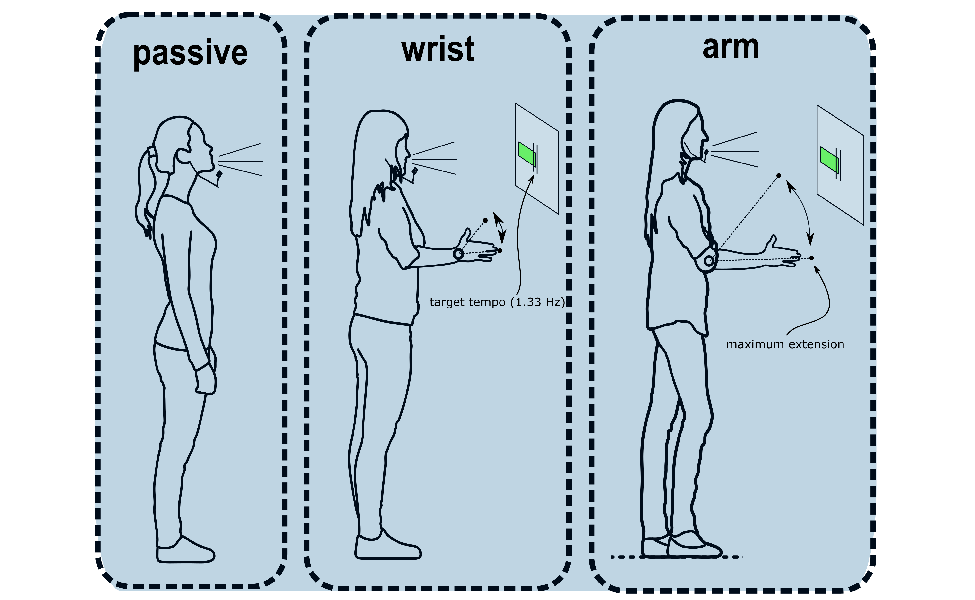
\includegraphics{GS_physics_in_fluid_speech_files/figure-latex/method_stance_pic-1} 

}

\end{figure}

\emph{Note}. Movement conditions are shown. Each participants performed all conditions (i.e., within-subjects). To ensure that movement tempo remained relatively constant participants were shown a moving green bar which indicated whether they moved to fast or to slow relative to a 20\% target region of 1.33Hz. Participants were instructed to have a emphasis in the downbeat with a abrupt stop (i.e., beat) at the maximum extension.

\hypertarget{preprocessing}{%
\subsection{Preprocessing}\label{preprocessing}}

\hypertarget{speech-acoustics}{%
\subsubsection{Speech acoustics}\label{speech-acoustics}}

The Fundamental Frequency was extracted with gender-appropriate preset ranges (male = 50-400Hz, female = 80-640Hz). We used a previously written (Pouw \& Trujillo, 2019) R-script (\url{https://osf.io/m43qy/}) utilizing R-package `wrassp' (Winkelmann, Bombien, \& Scheffers, 2018) which applies a K. Schaefer-Vincent algorithm. We also extracted a smoothed (5Hz hanning window) amplitude envelope using a previously written custom-written R script (\url{https://osf.io/uvkj6/}, which reimplements in R a procedure from He \& Dellwo (2017).

\hypertarget{data-and-exclusions}{%
\subsubsection{Data and Exclusions}\label{data-and-exclusions}}

Due to a c++ coding error the precise timing data for the motion-tracking was partially lost. This was caused by an incorrect memory allocation for a 7- instead of 8-digit vector in the c++ experiment code. This resulted in losing track of the tracking system's time above 1.000.000 milliseconds (16 min and 40 seconds). Thus the motion tracking data after 16m40s had to be excluded. Interpolation of missing time points for the remaining data was considered, but this will inevatably lead to temporal innacuracies as sampling rate of the recording system is never perfectly constant at 240Hz (as such a continuous time-keeping is needed). Thus if we only look at speech we will have access to all data, meaning 189.70 minutes of continous data (Passive = 63.45, Wrist Movement = 63.56, Arm Movement = 62.69). For analysis including kinematics, we have access to 124.49 minutes of continuous speech data (Passive = 40.08, Wrist Movement = 42.32, Arm Movement = 42.10).

\hypertarget{manipulation-checks}{%
\subsection{Manipulation Checks}\label{manipulation-checks}}

The following measures we computed as a way to check whether our movement manipulation was successful, and whether speech rates were comparable for conditions. Figure 2 shows a summary of the results for key manipulation check measures.

\hypertarget{movement-frequency}{%
\subsubsection{Movement Frequency}\label{movement-frequency}}

To ascertain if participants were indeed moving their limbs within the target range of 1.33Hz we performed a wavelet-based analysis with R-package `WaveletComp' (Rosch \& Schmidbauer, 2014), whereby we assessed for each time step which frequency had the highest estimated power (please see our processing script on OSF for further details). Figure 3. shows an example of the wavelet analysis, whereby faster osscilations indeed shower higher frequency estimates for that moment during the trial. It can be seen from Figure 2. that wrist movements were slightly performed at faster rates, \emph{M} = 1.44 Hz, \emph{SD} = 0.24, than arm movements, \emph{M} = 1.36 Hz, \emph{SD} = 0.19, but in both cases the movements were distributed over the range 1.33Hz. This confirms that our movement manipulation was succesful. Note further that for our surrogate control condition Passive (Falsely Paired) the mean frequency of the false movement time series was in between both Arm and Wrist movement frequency distributions, \emph{M} = 1.41 Hz, \emph{SD} = 0.22.

\hypertarget{speech-rate}{%
\subsubsection{Speech Rate}\label{speech-rate}}

For the current report we are interested in speech acoustics, and we will not go into a finegrained analysis of possible temporal changes of speech produced under rhythmic movement. However we have calculated two measures to provide an indication of speech rate (see Figure 2 for examples), namely vocalization duration and vocalization interval. Figure 3 shows relatively uniform distributions for speech measures, and thus no clear one-to-one frequency couplings of movement and vocalization duration/vocalization interval, or any other clear signs of polyrhythmic coupling of movement and speech as has been observed in basic tapping paradigms (Zelic et al., 2015).\\
We have computed the average vocalization duration for each trail by tracking the time of uninterrupted runs of F0 observations, and converted the time in milliseconds to Hz (cycles per second) so as to compare this measure to the the movement frequency distributions. For the Passive condition the average vocalization duration was \emph{M} = 3.99 Hz (i.e., 250ms), \emph{SD} = 5.68. For the Wrist condition the vocalization duration was \emph{M} = 4.19 Hz (i.e., 1000/3.99 = 250ms), \emph{SD} = 5.69, and for the Arm condition \emph{M} = 4.16 Hz (i.e., 250ms), \emph{SD} = 5.59.\\
The average vocalization interval for the Passive condition was \emph{M} = 5.17 Hz (i.e., 250ms), \emph{SD} = 6.94. For the Wrist condition the vocalization interval was \emph{M} = 5.02 Hz, \emph{SD} = 6.86, and for the Arm condition \emph{M} = 4.86 Hz, \emph{SD} = 5.76.

Figure 2. Example movement-, amplitude envelope-, F0- time series, and time-dependent movement frequency estimates
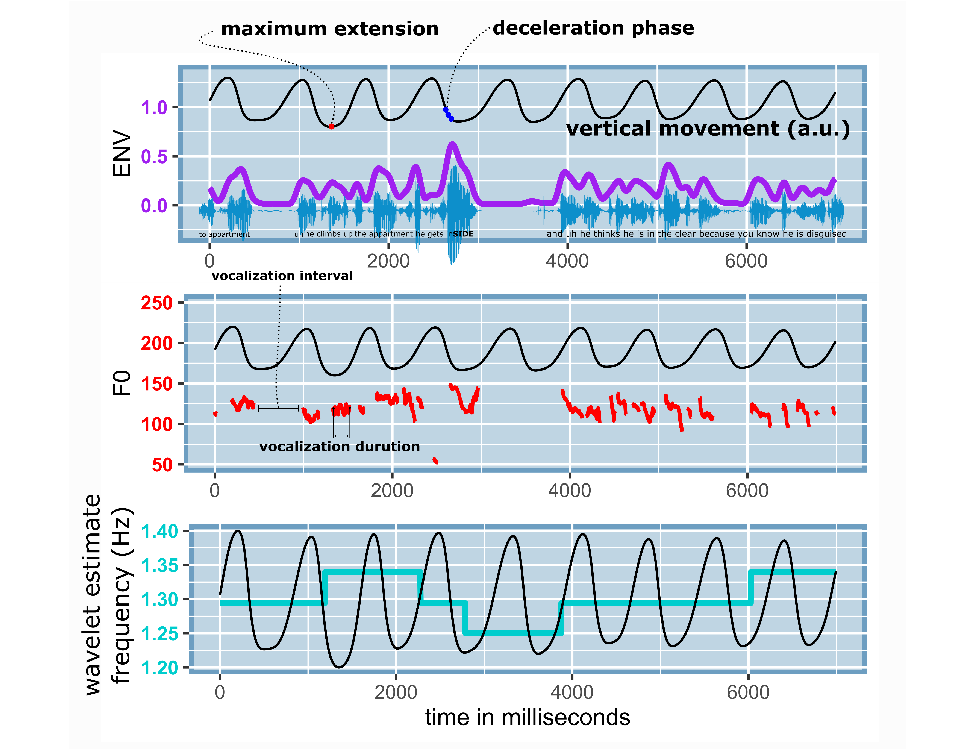
\includegraphics{GS_physics_in_fluid_speech_files/figure-latex/plot_example_time_series-1.pdf}

\emph{Note figure 2.} A sample of data of about 10 seconds is shown. With the participant's permission the speech sample is available at \url{https://osf.io/2qbc6/}. The amplitude envelope in purple traces smoothly the waveform maxima's. The F0 traces show the concomittant vocalizations in Hz, with an example of vocalization interval and vocalization duration (which was calcuated for all vocalizations). The bottom panel shows the continously estimated movement frequency in cyan, which hovers nicely around 1.33 Hz. In all these panels the co-occuring movement is plotted in arbitrary units (a.u.) so as see the temporal relation of movement phases and the amplitude envelope, F0, and the movement frequency estimate. Not that in our upcoming analysis we refer to the maximum extension and decelerration phases as relevant moments for speech modulations. In this example there is a particulary dramatic acoustic excursion during a moment of deceleration of the arm movement, possibly an example of gesture-speech physics.

Figure 3. Summary of movement-frequency, vocalization duration and vocalization interval

\includegraphics{GS_physics_in_fluid_speech_files/figure-latex/manipulation_check-1.pdf}
\emph{Note Figure 3}. Density distributions of movement frequencies, vocalization interval, and vocalization duration are shown. Note, that for the Passive condition there was no movement, but we have falsely paired movement time series for the Passive (Falsely Paired) condition for which frequency information is shown. The red vertical line indicates the target movement frequency at 1.3Hz.

\hypertarget{results}{%
\section{Results}\label{results}}

\hypertarget{overview-analysis}{%
\subsection{Overview analysis}\label{overview-analysis}}

We will report three main analysis to show that gesture-speech physics is present. Firstly, we will assess whether there are overall effects on movement condition on vocalization acoustics (F0 and the amplitude envelope). Secondly, we assess whether vocalization acoustic modulations are observed at particular phases of the movement condition. Thirdly, we assess whether continous estimate of upper limb forces produced, predicts vocalization acoustic peaks.\\
The following generally applies to all analysis: For hypothesis testing we performed mixed linear regression models with R-package `nlme' (Pinheiro, Bates, DebRoy, Sarkar, \& R Team, 2019), or non-linear generalized additive modeling (GAM) with R-package `gam' (Hastie, 2019) with random intercept for participants. If random slopes for any of the analysis converged as well we wil report so.

\hypertarget{acousic-correlates-of-movement-condition}{%
\subsection{Acousic correlates of movement condition}\label{acousic-correlates-of-movement-condition}}

Figure 4 shows the average F0 and Amplitude Envelope (z-scaled for participants) per trial per condition. It can be seen that the Passive condition had generally lower levels of F0 and Amplitude Envelope as compared to the movement conditions. Furthermore, the higher-impetus Arm condition generally had higher levels of F0 and Amplitude envelope as compared to lower-impetus Wrist condition.
Table 1 shows the results of mixed linear regression analysis. For the amplitude envelope,Passive condition had a lower average amplitude envelope as compared to the the Wrist condition (\emph{p} \textless{} .05), as well as the Arm condition (\emph{p} \textless{} .0001). We further obtain that after accounting for differences in F0 for gender (males had generally 73Hz lower F0), Wrist Movement condition has about 1.4 Hz increase in average (\emph{p} \textless{} .05) as compared to Passive condition. Further, the Arm movement condition had 3.2 Hz increase in F0 over the Passive Condition (\emph{p} \textless{} .0001).

Figure 4. Average F0 and Amplitude Envelope per trial per condition.

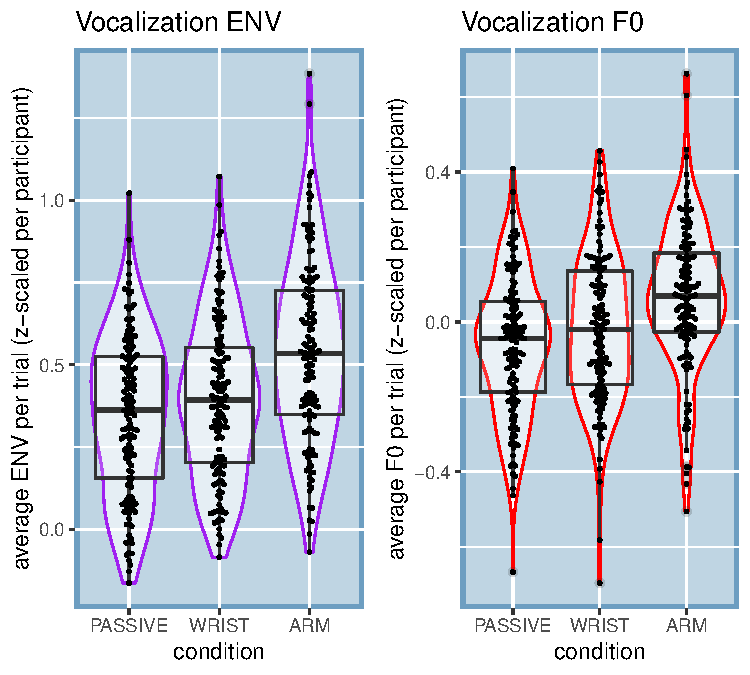
\includegraphics{GS_physics_in_fluid_speech_files/figure-latex/plot_avF0_avENV-1.pdf}

\emph{Note Figure 4}. Violin and box plots are shown for average F0 (Hz) and amplitude envelope (z-scaled) per trial (jitters show observation).

\pagebreak

Table 1. Linear mixed effects for effects of condition on F0 and Amplitude envelope

\begin{tabular}{lccccc}
\toprule
  & contrast & b & SE & df & p\\
\midrule
ENV (z-scaled) & intercept & 0.347 & 0.033 & 382 & < .0001\\
 & Wrist vs. Passive & 0.048 & 0.022 & 382 & 0.0287\\
 & Arm vs. Passive & 0.189 & 0.022 & 382 & < .0001\\
 &  &  &  &  & \\
F0 (Hz) & intercept & 186.916 & 3.25 & 382 & < .0001\\
\addlinespace
 & Male vs. Female & -73.049 & 5.511 & 33 & < .0001\\
 & Wrist vs. Passive & 1.419 & 0.673 & 382 & 0.0357\\
 & Arm vs. Passive & 3.208 & 0.674 & 382 & < .0001\\
\bottomrule
\end{tabular}

\hypertarget{coupling-of-vocalization-duration-and-movement}{%
\subsection{Coupling of vocalization duration and movement}\label{coupling-of-vocalization-duration-and-movement}}

Having ascertained in the previous analysis that there seem to be acoustic modulations for movement versus no movement, we further need to confirm that such modulations occur at particular moments. Namely, we have previously obtained that acoustic effects arise at moments around the maximum extension where the most forceful changes in speed (i.e., deceleration/acceleration) are observed.
Figure 5 shows the main results. It can be seen that just before the moment of maximum extension that there is a clear peak in the observed amplitude envelope, most dramatically for Arm condition, but also present for the Wrist condition. For falsely paired movement and passive condition speech this was not the case, excluding mere chance occurences. For F0 more complex patterns are shown, but still with positive peaks just before the maximum extension. This nicely replicates our earlier work on steady-state vocalization, showing that at moments of peak deceleration there are observed peaks in acoustics (Pouw et al., 2019b).
To formally test that trajectories are indeed non-linear and are reliably different from the passive condition, we performed GAM, a type of non-linear mixed effects procedure. We assessed the average trajectory of acoustics around 800 milliseconds of the maximum extension of the mvoement. We chose 800 milliseconds as this is about the time for a 1.3Hz cycle. The model results with random slopes and intercept for participant are shown in table 2. Firstly, for all models tests for non-linearity of the trajectories were statistically reliable (\emph{p}'s \textless{} .0001). As shown in Table 2 our results replicate the general finding that Wrist movements lead to reliably different non-linear peaks in acoustics as compared to the passive condition (\emph{p} \textless{} .0001), and this effect is even more extreme for the Arm movement condition (\emph{p} \textless{} .0001). Figure 6 provides the fitted trajectories for the GAM models.\\
For readers interested in individual differences in trajectories, we have uploaded an interactive graph where each participant's average Amplitude Envelope trajectories can be inspected (\url{https://osf.io/a423h/}), as well for F0 trajectories (\url{https://osf.io/fdzwj/}).
\pagebreak
Figure 5. Average observed vocalization acoustics relative to the moment of maximum extension\\
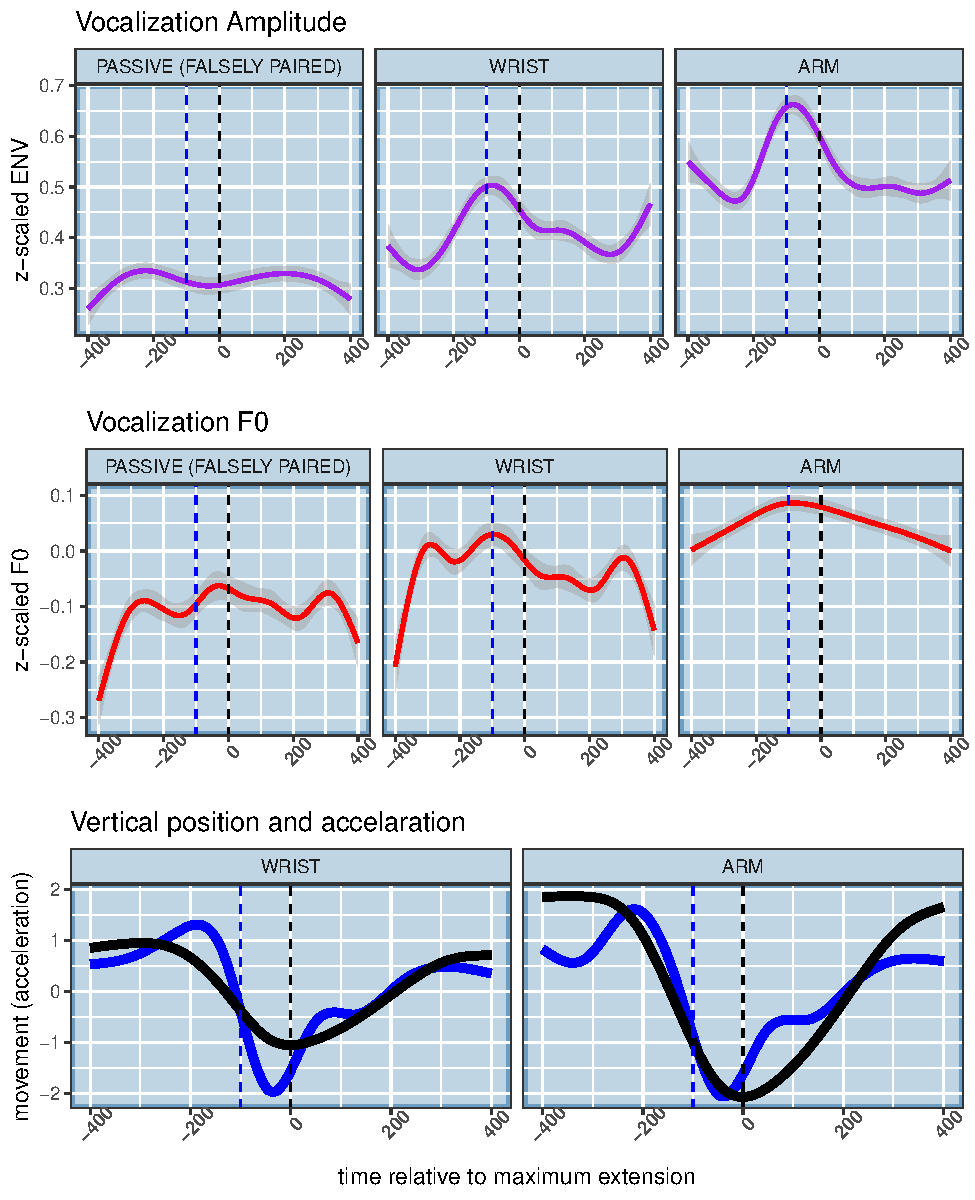
\includegraphics{GS_physics_in_fluid_speech_files/figure-latex/movementplot_avF0_avENV-1.pdf}

\emph{Note Figure 5}. For the upper two panels the average acoustic trajectory is shown around the moment of maximum extension (\emph{t} = 0, dashed line). In the lower panel we have plotted the z-scaled average vertical displacement of the hand, and the z-scaled acceleration trace. We have marked with the blue dashed vertical line the moment where the deceleration phase starts, which neatly alligns with peaks in acoustics.

Figure 6. Fitted trajectories GAM
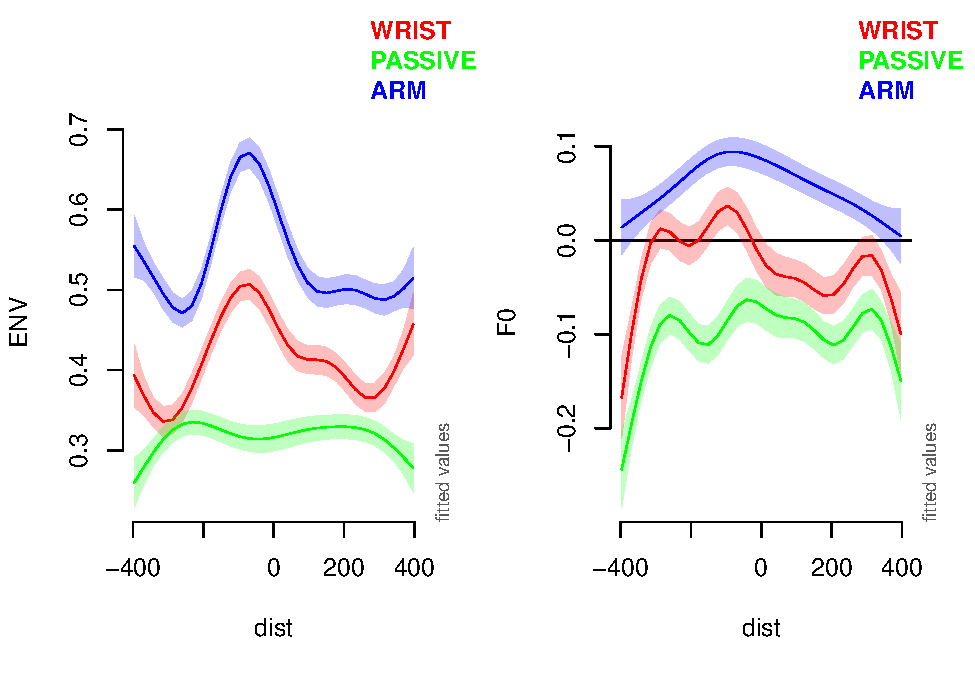
\includegraphics{GS_physics_in_fluid_speech_files/figure-latex/table_anddiff-1.pdf}

Table 2. Model results for GAM analysis

\begin{tabular}{lccccc}
\toprule
  & contrast & b & SE & df & p\\
\midrule
ENV (z-scaled) & intercept & 0.237 & 0.006 & 36.923 & < .0001\\
 & Wrist vs. Passive & 0.096 & 0.009 & 10.579 & < .0001\\
 & Arm vs. Passive & 0.152 & 0.009 & 16.862 & < .0001\\
 &  &  &  &  & \\
F0 (Hz) & intercept & -0.061 & 0.006 & -8.351 & < .0001\\
\addlinespace
 & Male vs. Female & -0.019 & 0.009 & -4.29 & < .0001\\
 & Wrist vs. Passive & 0.101 & 0.009 & 10.222 & < .0001\\
 & Arm vs. Passive & 0.094 & 0.103 & 9.546 & < .0001\\
\bottomrule
\end{tabular}

\emph{Note}. Model results are shown for the ampltiude envelope (z-scaled) and F0 (Hz). For F0 we accounted for differences of gender when estimating independent effects of condition.

\hypertarget{degree-of-physical-impetus-and-acoustic-peaks}{%
\subsection{Degree of physical impetus and acoustic peaks}\label{degree-of-physical-impetus-and-acoustic-peaks}}

We have confirmed that speech acoustics is modulated around moments of the deceleration phase, about 0-200 ms before the maximum extension. However a further support of gesture-speech physics would entail a demonstration that forces produced by the upper limb movement predict acoustic peaks. Therefore we assessed for all vocalizations that occurred between 200 to 0ms before the maximum extension whether its acoustic peak (maximum F0 or maximum amplitude envelope) was predicted by the maximum deceleration value (i.e, minimum acceleration observation) observed in that 200 millisecond window. In previous research we obtained that higher deceleration were related to higher amplitude envelope observations, but not F0 (Pouw et al., 2019a).
Figure 7 shows the general pattern of the results for the Wrist and Arm condition. Table 3 shows the results of linear mixed effects model with random intercept and slopes for participants, where we regressed the max observation deceleration onto the co-occuring vocalization acoustic peak, for amplitude envelope and F0 seperately. We observed that higher deceleration was indeed predicting higher amplitude envelope, for both Wrist and Arm movements (\emph{p} \textless{} .001). Similar to previous research, for F0 this effect is much more weakly present, and only for the Arm movement condition, as indicated by a statistically reliable interaction between condition and max deceleration effect (\emph{p} \textless{} .05).

Figure 7. Relation max deceleration and height acoustic peak
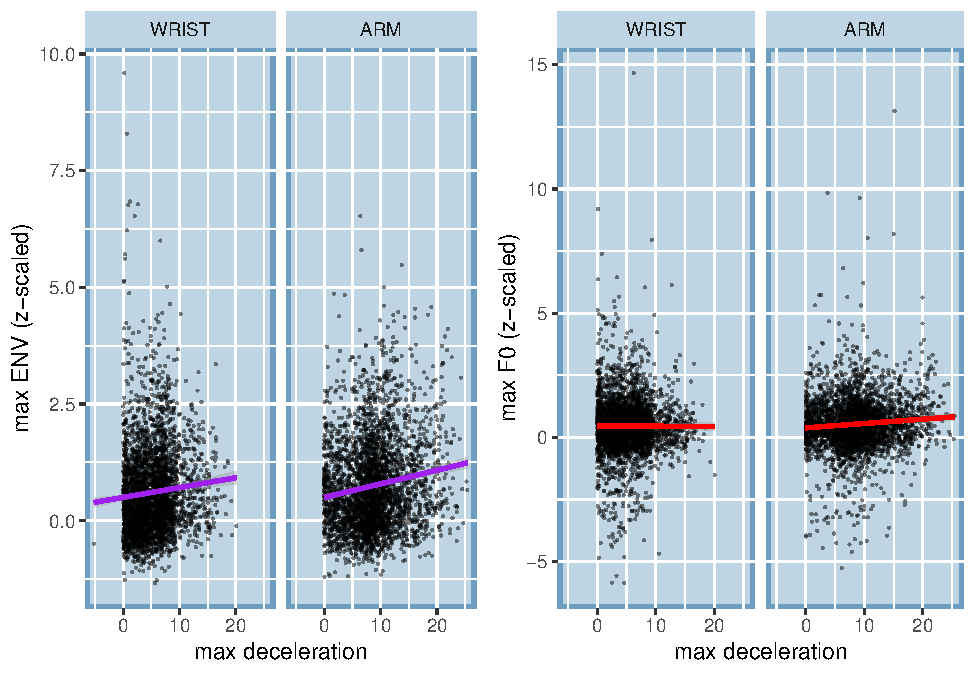
\includegraphics{GS_physics_in_fluid_speech_files/figure-latex/impact analysis-1.pdf}

\emph{Note Figure 7}. On the x-axis the maximum deceleration is shown (absolutized negative acceleration value), where 0 indicates no deceleration and positive values indicate higher deceration rates in cm/s. It can be seen that deceleration rates are more extreme for the Arm versus the Wrist condition. On the y-axis we have maximum observed amplitude envelope (left panel) and F0 around that moment of deceleration. There is a general trend that higher decelerations are co-occur with higher peaks in acoustics, especially for the amplitude envelope, and especially for the Arm condition.\\
\newpage

Table 4. Linear mixed effects of deceleration and acoustic peaks

\begin{tabular}{lccccc}
\toprule
  & contrast & b & SE & df & p\\
\midrule
ENV (z-scaled) & Intercept & 0.427 & 0.05 & 6711 & < .0001\\
 & Arm vs. Wrist & 0.001 & 0.026 & 6711 & 0.9593\\
 & Max Deceleration & 0.039 & 0.006 & 6711 & < .0001\\
 &  &  &  &  & \\
F0 (z-scaled) & intercept & 0.441 & 0.046 & 6709 & < .0001\\
\addlinespace
 & Arm vs. Wrist & -0.064 & 0.054 & 6709 & 0.2417\\
 & Max Deceleration & 0.001 & 0.006 & 6709 & 0.8767\\
 & Arm x Max Deceleration & 0.017 & 0.007 & 6709 & 0.0178\\
\bottomrule
\end{tabular}

\emph{Note}. We included interaction terms if they were found to be statistically reliable.

\pagebreak

\hypertarget{discussion}{%
\section{Discussion}\label{discussion}}

The current study concludes on a line of research demonstrating biomechanical effects of gesture onto speech, by replicating effects obtained in steady-state vocalization and mono-syllable utterances in fluid speech. We show that rhythmically moving the wrist or arm, affects vocalization acoustics by heightening F0 and amplitude envelope, as compared to a passive control condition. We further show that acoustic modulations are especially found around moments of the high-impetus beat, i.e., where the movement abruptly decelerates, thereby producing a physical impetus on the body. We finally show that higher deceleration rates of the movement materialize into more extreme acoustic peaks, demonstrating a role for force-transmission from gesture onto speech. In all analysis we observe that higher-impetus arm versus wrist movements affects speech more dramatically.\\
The current study opens up a line of possible research into understanding how biomechanics are counteracted or exploited depending the speakers intentions and information structure of the utterances. Indeed, it should be noted that gesture-speech physics have only been explicitly tested in situations where participants are instructed to keep their vocalizations or speech as stable as possible. Although a recent study did show that encouraging participants to gesture, without any instruction on how to speak, did lead to modulation of acoustics similar to the current (Cravotta et al., 2019). In the current study, however, participants are likely to counteract effects of the movements. Future research should therefore focus on how prosodic goals might recruit biomechanical resources. Indeed, although the movements may have been experienced as a nuisance for participants in the current experiment, we would maintain that gesture-speech physics is a \emph{resource} that can be recruited by an embodied speaker. Prosodic goals, such as producing a pitch accent, can thereby be in part performed by a `morphological computation' (Zhang \& Ghazanfar, 2018), i.e., producing a physical impetus on lower vocal tract via gesturing.\\
If the current line of research is on track we can conclude that gesture and speech are by biomehanical necessity coupled. This means that when moving the upper limbs this will constrain vocalization acoustics. This by no means entails a non-cognitive or a `dumb' by-product of our bodies that are cognitively non-negotiable. Rather, biomechanics such as these are providing behavioral stabilities that can be allowed by the speaker to arise, and which would be more complicated to perform by some other sensorimotor solution (Perrier \& Fuchs, 2015). We have argued in this respect that cognitively, the biomehechanical coupling of gesture and speech provides a `smart' mechanism for `timing' acoustic and movement expressions. With regards to ontogenesis of gesture-speech coupling, we think gesture-speech physics explains how an infant learns to produce multimodal utterances, through the natural discovery of morphological computations during kinesthetic exploration in the form of vocal-motor babbling (Ejiri, 1998). Phylogenetically, gesture-speech physics may have shaped the evolution of the vocal system in humans and may have been a not-yet considered driver for why gesture and speech are now a ubiqituously exploited sensorimotor coalition in our species. What makes this particular thesis exciting we think, is that all theories on multimodal language evolution have been preoccupied with showing how representational functions of gesture are the primary reason for multimodal language to exist, piggybacking on arguably shaky bets that such representational gestural capacities are also present in some proto-form in non-human homonids (Corballis, 2002; Fröhlich et al., 2019; Kendon, 2017; Levinson \& Holler, 2014; Prieur et al., 2019; Tomasello, 2008). Perhaps then, gesture-speech physics provides a more solid primordial basis for the evolution of multimodal behavior, whereby peripheral bodily tensioning naturally formed coalitions with sound-producing organs that were still very much under development. A particularly needed theoretical enterprise for such an radically embodied revision of the origins of multimodal behavior would therefore be to reconsider whether multimodal behavior can be connected to the wider cross-species literature on bioacoustics showing a more widespread existence of embodied innovations for communication similar to the current (Ghazanfar, 2013; Hardus et al., 2009; Larsson et al., 2019; Pouw et al., 2019d; Ravignani et al., 2019).
\newpage

\hypertarget{references}{%
\section{References}\label{references}}

\begingroup
\setlength{\parindent}{-0.5in}
\setlength{\leftskip}{0.5in}

\hypertarget{refs}{}
\begin{cslreferences}
\leavevmode\hypertarget{ref-cooperriderForegroundGestureBackground2019}{}%
Cooperrider, K. (2019). Foreground gesture, background gesture. \emph{Gesture}, \emph{16}(2), 176--202. doi:\href{https://doi.org/https://doi.org/10.1075/gest.16.2.02coo}{https://doi.org/10.1075/gest.16.2.02coo}

\leavevmode\hypertarget{ref-corballisHandMouthOrigins2002}{}%
Corballis, M. C. (2002). \emph{From hand to mouth: The origins of language}. Princeton, NJ.: Princeton University Press.

\leavevmode\hypertarget{ref-cordoPropertiesPosturalAdjustments1982}{}%
Cordo, P. J., \& Nashner, L. M. (1982). Properties of postural adjustments associated with rapid arm movements. \emph{Journal of Neurophysiology}, \emph{47}(2), 287--302. doi:\href{https://doi.org/10.1152/jn.1982.47.2.287}{10.1152/jn.1982.47.2.287}

\leavevmode\hypertarget{ref-cravottaEffectsEncouragingUse2019}{}%
Cravotta, A., Busà, M. G., \& Prieto, P. (2019). Effects of Encouraging the Use of Gestures on Speech. \emph{Journal of Speech, Language, and Hearing Research}. doi:\href{https://doi.org/10.21437/SpeechProsody.2018-42}{10.21437/SpeechProsody.2018-42}

\leavevmode\hypertarget{ref-dannerQuantitativeAnalysisMultimodal2018}{}%
Danner, S. G., Barbosa, A. V., \& Goldstein, L. (2018). Quantitative analysis of multimodal speech data. \emph{Journal of Phonetics}, \emph{71}, 268--283. doi:\href{https://doi.org/10.1016/j.wocn.2018.09.007}{10.1016/j.wocn.2018.09.007}

\leavevmode\hypertarget{ref-ejiriRelationshipRhythmicBehavior1998}{}%
Ejiri, K. (1998). Relationship between Rhythmic Behavior and Canonical Babbling in Infant Vocal Development. \emph{Phonetica}, \emph{55}(4), 226--237. doi:\href{https://doi.org/10.1159/000028434}{10.1159/000028434}

\leavevmode\hypertarget{ref-ejiriCooccurencesPreverbalVocal2001}{}%
Ejiri, K., \& Masataka, N. (2001). Co-occurences of preverbal vocal behavior and motor action in early infancy. \emph{Developmental Science}, \emph{4}(1), 40--48. doi:\href{https://doi.org/10.1111/1467-7687.00147}{10.1111/1467-7687.00147}

\leavevmode\hypertarget{ref-esteve-gibertProsodicStructureShapes2013}{}%
Esteve-Gibert, N., \& Prieto, P. (2013). Prosodic structure shapes the temporal Realization of intonation and manual gesture movements. \emph{Journal of Speech, Language, and Hearing Research}, \emph{56}(3), 850--864. doi:\href{https://doi.org/10.1044/1092-4388(2012/12-0049)}{10.1044/1092-4388(2012/12-0049)}

\leavevmode\hypertarget{ref-feyereisenCognitivePsychologySpeechRelated2017}{}%
Feyereisen, P. (2017). \emph{The Cognitive Psychology of Speech-Related Gesture}. New York: Routledge. Retrieved from \url{http://books.google.com?id=nJguDwAAQBAJ}

\leavevmode\hypertarget{ref-frohlichMultimodalCommunicationLanguage2019}{}%
Fröhlich, M., Sievers, C., Townsend, S. W., Gruber, T., \& Schaik, C. P. van. (2019). Multimodal communication and language origins: Integrating gestures and vocalizations. \emph{Biological Reviews}, \emph{94}(5), 1809--1829. doi:\href{https://doi.org/10.1111/brv.12535}{10.1111/brv.12535}

\leavevmode\hypertarget{ref-gardenforsDemonstrationPantomimeEvolution2017}{}%
Gärdenfors, P. (2017). Demonstration and Pantomime in the Evolution of Teaching. \emph{Frontiers in Psychology}, \emph{8}. doi:\href{https://doi.org/10.3389/fpsyg.2017.00415}{10.3389/fpsyg.2017.00415}

\leavevmode\hypertarget{ref-ghazanfarMultisensoryVocalCommunication2013}{}%
Ghazanfar, A. A. (2013). Multisensory vocal communication in primates and the evolution of rhythmic speech. \emph{Behavioral Ecology and Sociobiology}, \emph{67}(9). doi:\href{https://doi.org/10.1007/s00265-013-1491-z}{10.1007/s00265-013-1491-z}

\leavevmode\hypertarget{ref-ghazanfarVocaltractResonancesIndexical2007}{}%
Ghazanfar, A. A., Turesson, H. K., Maier, J. X., van Dinther, R., Patterson, R. D., \& Logothetis, N. K. (2007). Vocal-tract resonances as indexical cues in rhesus monkeys. \emph{Current Biology}, \emph{17}(5-2), 425--430. doi:\href{https://doi.org/10.1016/j.cub.2007.01.029}{10.1016/j.cub.2007.01.029}

\leavevmode\hypertarget{ref-ginosarLearningIndividualStyles2019}{}%
Ginosar, S., Bar, A., Kohavi, G., Chan, C., Owens, A., \& Malik, J. (2019). Learning individual styles of conversational gesture. In \emph{Proceedings of the IEEE Conference on Computer Vision and Pattern Recognition} (pp. 3497--3506). Retrieved from \url{https://arxiv.org/abs/1906.04160}

\leavevmode\hypertarget{ref-hardusToolUseWild2009}{}%
Hardus, M. E., Lameira, A. R., Schaik, C. S., \& Wich, S. A. (2009). Tool use in wild orang-utans modifies sound production: A functionally deceptive innovation? \emph{Proceedings of the Royal Society B: Biological Sciences}, \emph{276}(1673), 3689--3694. doi:\href{https://doi.org/10.1098/rspb.2009.1027}{10.1098/rspb.2009.1027}

\leavevmode\hypertarget{ref-hastieGamGeneralizedAdditive2019}{}%
Hastie, T. (2019). Gam: Generalized Additive Models (Version 1.16.1). Retrieved from \url{https://CRAN.R-project.org/package=gam}

\leavevmode\hypertarget{ref-heAmplitudeEnvelopeKinematics2017a}{}%
He, L., \& Dellwo, V. (2017). Amplitude envelope kinematics of speech: Parameter extraction and applications. \emph{The Journal of the Acoustical Society of America}, \emph{141}(5), 3582--3582. doi:\href{https://doi.org/10.1121/1.4987638}{10.1121/1.4987638}

\leavevmode\hypertarget{ref-hollerMultimodalLanguageProcessing2019}{}%
Holler, J., \& Levinson, S. C. (2019). Multimodal language processing in human communication. \emph{Trends in Cognitive Sciences}, \emph{23}(8), 639--652. doi:\href{https://doi.org/10.1016/j.tics.2019.05.006}{10.1016/j.tics.2019.05.006}

\leavevmode\hypertarget{ref-iversonHandMouthBrain2005}{}%
Iverson, J. M., \& Thelen, E. (2005). Hand, mouth and brain: The dynamic emergence of speech and gesture. \emph{Journal of Consciousness Studies}, 22.

\leavevmode\hypertarget{ref-kelsoConvergingEvidenceSupport1984}{}%
Kelso, J. A., \& Tuller, B. (1984). Converging evidence in support of common dynamical principles for speech and movement coordination. \emph{The American Journal of Physiology}, \emph{246}(6 Pt 2), R928--935. doi:\href{https://doi.org/10.1152/ajpregu.1984.246.6.R928}{10.1152/ajpregu.1984.246.6.R928}

\leavevmode\hypertarget{ref-kendonReflectionsGesturefirstHypothesis2017}{}%
Kendon, A. (2017). Reflections on the ``gesture-first'' hypothesis of language origins. \emph{Psychonomic Bulletin \& Review}, \emph{24}(1), 163--170. doi:\href{https://doi.org/10.3758/s13423-016-1117-3}{10.3758/s13423-016-1117-3}

\leavevmode\hypertarget{ref-kitaPointingWhereLanguage2003}{}%
Kita, S. (2003). \emph{Pointing: Where language, culture, and cognition meet}. Mahwah, NJ, US: Lawrence Erlbaum Associates Publishers.

\leavevmode\hypertarget{ref-krahmerEffectsVisualBeats2007}{}%
Krahmer, E., \& Swerts, M. (2007). The effects of visual beats on prosodic prominence: Acoustic analyses, auditory perception and visual perception. \emph{Journal of Memory and Language}, \emph{57}(3), 396--414. doi:\href{https://doi.org/10.1016/j.jml.2007.06.005}{10.1016/j.jml.2007.06.005}

\leavevmode\hypertarget{ref-krivokapicGesturalCoordinationProsodic2014}{}%
Krivokapić, J. (2014). Gestural coordination at prosodic boundaries and its role for prosodic structure and speech planning processes. \emph{Philosophical Transactions of the Royal Society B: Biological Sciences}, \emph{369}(1658). doi:\href{https://doi.org/10.1098/rstb.2013.0397}{10.1098/rstb.2013.0397}

\leavevmode\hypertarget{ref-krivokapicKinematicStudyProsodic2017}{}%
Krivokapić, J., Tiede, M. K., \& Tyrone, M. E. (2017). A Kinematic Study of Prosodic Structure in Articulatory and Manual Gestures: Results from a Novel Method of Data Collection. \emph{Laboratory Phonology: Journal of the Association for Laboratory Phonology}, \emph{8}(1), 3. doi:\href{https://doi.org/10.5334/labphon.75}{10.5334/labphon.75}

\leavevmode\hypertarget{ref-kucherenkoAnalyzingInputOutput2019}{}%
Kucherenko, T., Hasegawa, D., Henter, G. E., Kaneko, N., \& Kjellström, H. (2019). Analyzing Input and Output Representations for Speech-Driven Gesture Generation. In \emph{Proceedings of the 19th ACM International Conference on Intelligent Virtual Agents - IVA '19} (pp. 97--104). Paris, France: ACM Press. doi:\href{https://doi.org/10.1145/3308532.3329472}{10.1145/3308532.3329472}

\leavevmode\hypertarget{ref-lancasterRespiratoryMuscleActivity1995}{}%
Lancaster, W. C., Henson, O. W., \& Keating, A. W. (1995). Respiratory muscle activity in relation to vocalization in flying bats. \emph{Journal of Experimental Biology}, \emph{198}(1), 175--191. Retrieved from \url{https://jeb.biologists.org/content/198/1/175}

\leavevmode\hypertarget{ref-larssonBipedalStepsDevelopment2019}{}%
Larsson, M., Richter, J., \& Ravignani, A. (2019). Bipedal Steps in the Development of Rhythmic Behavior in Humans. \emph{Music \& Science}, \emph{2}, 2059204319892617. doi:\href{https://doi.org/10.1177/2059204319892617}{10.1177/2059204319892617}

\leavevmode\hypertarget{ref-leonardTemporalRelationBeat2011}{}%
Leonard, T., \& Cummins, F. (2011). The temporal relation between beat gestures and speech. \emph{Language and Cognitive Processes}, \emph{26}(10), 1457--1471. doi:\href{https://doi.org/10.1080/01690965.2010.500218}{10.1080/01690965.2010.500218}

\leavevmode\hypertarget{ref-levinsonOriginHumanMultimodal2014}{}%
Levinson, S. C., \& Holler, J. (2014). The origin of human multi-modal communication. \emph{Philosophical Transactions of the Royal Society B: Biological Sciences}, \emph{369}(1651). doi:\href{https://doi.org/10.1098/rstb.2013.0302}{10.1098/rstb.2013.0302}

\leavevmode\hypertarget{ref-loehrTemporalStructuralPragmatic2012}{}%
Loehr, D. P. (2012). Temporal, structural, and pragmatic synchrony between intonation and gesture. \emph{Laboratory Phonology}, \emph{3}(1), 71--89. doi:\href{https://doi.org/10.1515/lp-2012-0006}{10.1515/lp-2012-0006}

\leavevmode\hypertarget{ref-mcclavePitchManualGestures1998}{}%
McClave, E. (1998). Pitch and Manual Gestures. \emph{Journal of Psycholinguistic Research}, \emph{27}(2), 69--89. doi:\href{https://doi.org/https://doi.org/10.1023/A:1023274823974}{https://doi.org/10.1023/A:1023274823974}

\leavevmode\hypertarget{ref-mendoza-dentonSemioticLayeringGesture2011}{}%
Mendoza-Denton, N., \& Jannedy, S. (2011). Semiotic Layering through Gesture and Intonation: A Case Study of Complementary and Supplementary Multimodality in Political Speech. \emph{Journal of English Linguistics}, \emph{39}(3), 265--299. doi:\href{https://doi.org/10.1177/0075424211405941}{10.1177/0075424211405941}

\leavevmode\hypertarget{ref-parrellSpatiotemporalCouplingSpeech2014}{}%
Parrell, B., Goldstein, L., Lee, S., \& Byrd, D. (2014). Spatiotemporal coupling between speech and manual motor actions. \emph{Journal of Phonetics}, \emph{42}, 1--11. doi:\href{https://doi.org/10.1016/j.wocn.2013.11.002}{10.1016/j.wocn.2013.11.002}

\leavevmode\hypertarget{ref-perrierMotorEquivalenceSpeech2015}{}%
Perrier, P., \& Fuchs, S. (2015). Motor Equivalence in Speech Production. In \emph{The Handbook of Speech Production} (pp. 223--247). John Wiley \& Sons, Ltd. doi:\href{https://doi.org/10.1002/9781118584156.ch11}{10.1002/9781118584156.ch11}

\leavevmode\hypertarget{ref-pinheiroNlmeLinearNonlinear2019}{}%
Pinheiro, J., Bates, D., DebRoy, S., Sarkar, D., \& R Team, R. C. (2019). \emph{Nlme: Linear and nonlinear mixed effects models}.

\leavevmode\hypertarget{ref-pisanskiVoiceModulationWindow2016}{}%
Pisanski, K., Cartei, V., McGettigan, C., Raine, J., \& Reby, D. (2016a). Voice modulation: A window into the origins of guman vocal control? \emph{Trends in Cognitive Sciences}, \emph{20}(4), 304--318. doi:\href{https://doi.org/10.1016/j.tics.2016.01.002}{10.1016/j.tics.2016.01.002}

\leavevmode\hypertarget{ref-pisanskiReturnOzVoice2014}{}%
Pisanski, K., Fraccaro, P. J., Tigue, C. C., O'Connor, J. J. M., \& Feinberg, D. R. (2014). Return to Oz: Voice pitch facilitates assessments of men's body size. \emph{Journal of Experimental Psychology. Human Perception and Performance}, \emph{40}(4), 1316--1331. doi:\href{https://doi.org/10.1037/a0036956}{10.1037/a0036956}

\leavevmode\hypertarget{ref-pisanskiCanBlindPersons2016}{}%
Pisanski, K., Oleszkiewicz, A., \& Sorokowska, A. (2016b). Can blind persons accurately assess body size from the voice? \emph{Biology Letters}, \emph{12}(4), 20160063. doi:\href{https://doi.org/10.1098/rsbl.2016.0063}{10.1098/rsbl.2016.0063}

\leavevmode\hypertarget{ref-pouwEntrainmentModulationGesture2019}{}%
Pouw, W., \& Dixon, J. A. (2019a). Entrainment and modulation of gesture--speech synchrony under delayed auditory feedback. \emph{Cognitive Science}, \emph{43}(3), e12721. doi:\href{https://doi.org/10.1111/cogs.12721}{10.1111/cogs.12721}

\leavevmode\hypertarget{ref-pouwQuantifyingGesturespeechSynchrony2019}{}%
Pouw, W., \& Dixon, J. A. (2019b). Quantifying gesture-speech synchrony. In \emph{Proceedings of the 6th meeting of Gesture and Speech in Interaction} (pp. 68--74). Paderborn: Universitaetsbibliothek Paderborn. doi:\href{https://doi.org/10.17619/UNIPB/1-812}{10.17619/UNIPB/1-812}

\leavevmode\hypertarget{ref-pouwEnergyFlowsGesturespeech2019a}{}%
Pouw, W., Esteve-Gibert, N., Harrison, S. H., \& Dixon, J. A. (2019a). \emph{Energy flows in gesture-speech physics: The respiratory-vocal system and its coupling with hand gestures}. Retrieved from \url{https://psyarxiv.com/rnpav}

\leavevmode\hypertarget{ref-pouwGesturespeechPhysicsBiomechanical2019}{}%
Pouw, W., Harrison, S. H., \& Dixon, J. A. (2019b). Gesture-speech physics: The biomechanical basis of the emergence of gesture-speech synchrony. \emph{Journal of Experimental Psychology: General}. doi:\href{https://doi.org/10.1037/xge0000646}{10.1037/xge0000646}

\leavevmode\hypertarget{ref-pouwAcousticSpecificationUpper2019}{}%
Pouw, W., Paxton, A., Harrison, S. J., \& Dixon, J. A. (2019c). Acoustic specification of upper limb movement in voicing. In \emph{Proceedings of the 6th meeting of Gesture and Speech in Interaction} (pp. 75--80). Paderborn, Germany: Universitaetsbibliothek Paderborn. doi:\href{https://doi.org/10.17619/UNIPB/1-812}{10.17619/UNIPB/1-812}

\leavevmode\hypertarget{ref-pouwSocialResonanceAcoustic2019}{}%
Pouw, W., Paxton, A., Harrison, S. J., \& Dixon, J. A. (2019d). \emph{Social Resonance: Acoustic Information about Upper Limb Movement in Voicing}. Retrieved from \url{https://psyarxiv.com/ny39e}

\leavevmode\hypertarget{ref-pouwMaterialsTutorialGespin20192019}{}%
Pouw, W., \& Trujillo, J. P. (2019). \emph{Materials Tutorial Gespin2019 - Using video-based motion tracking to quantify speech-gesture synchrony}. Retrieved from \url{10.17605/OSF.IO/RXB8J}

\leavevmode\hypertarget{ref-prieurOriginsGesturesLanguage2019}{}%
Prieur, J., Barbu, S., Blois-Heulin, C., \& Lemasson, A. (2019). The origins of gestures and language: History, current advances and proposed theories. \emph{Biological Reviews of the Cambridge Philosophical Society}. doi:\href{https://doi.org/10.1111/brv.12576}{10.1111/brv.12576}

\leavevmode\hypertarget{ref-ravignaniRhythmSpeechAnimal2019}{}%
Ravignani, A., Dalla Bella, S., Falk, S., Kello, C. T., Noriega, F., \& Kotz, S. (2019). Rhythm in speech and animal vocalizations: A cross‐species perspective. \emph{Annals of the New York Academy of Sciences}. doi:\href{https://doi.org/10.1111/nyas.14166}{10.1111/nyas.14166}

\leavevmode\hypertarget{ref-rochet-capellanSpeechFocusPosition2008}{}%
Rochet-Capellan, A., Laboissière, R., Galván, A., \& Jean-Luc, S. (2008). The speech focus position effect on jaw--finger coordination in a pointing task. \emph{Journal of Speech, Language, and Hearing Research}, \emph{51}(6), 1507--1521. doi:\href{https://doi.org/10.1044/1092-4388(2008/07-0173)}{10.1044/1092-4388(2008/07-0173)}

\leavevmode\hypertarget{ref-roschWaveletCompGuidedTour2014}{}%
Rosch, A., \& Schmidbauer, H. (2014). WaveletComp 1.1: A guided tour through the R package, 59.

\leavevmode\hypertarget{ref-ruiterProductionGestureSpeech2000}{}%
Ruiter, J. P. de. (2000, August). \emph{The production of gesture and speech}. \emph{Language and Gesture}. doi:\href{https://doi.org/10.1017/CBO9780511620850.018}{10.1017/CBO9780511620850.018}

\leavevmode\hypertarget{ref-silvaSteadystateStressOne2007}{}%
Silva, P., Moreno, M., Mancini, M., Fonseca, S., \& Turvey, M. T. (2007). Steady-state stress at one hand magnifies the amplitude, stiffness, and non-linearity of oscillatory behavior at the other hand. \emph{Neuroscience Letters}, \emph{429}(1), 64--68. doi:\href{https://doi.org/10.1016/j.neulet.2007.09.066}{10.1016/j.neulet.2007.09.066}

\leavevmode\hypertarget{ref-stoltmannSyllablepointingGestureCoordination2017}{}%
Stoltmann, K., \& Fuchs, S. (2017). Syllable-pointing gesture coordination in Polish counting out rhymes: The effect of speech rate. \emph{Journal of Multimodal Communication Studies}, \emph{4}(1-2), 63--68.

\leavevmode\hypertarget{ref-streeckDepictingGesture2008}{}%
Streeck, J. (2008). Depicting by gesture. \emph{Gesture}, \emph{8}(3), 285--301. doi:\href{https://doi.org/10.1075/gest.8.3.02str}{10.1075/gest.8.3.02str}

\leavevmode\hypertarget{ref-tomaselloOriginsHumanCommunication2008}{}%
Tomasello, M. (2008). \emph{The origins of human communication}. Cambdride, MA: MIT press.

\leavevmode\hypertarget{ref-treffnerIntentionalAttentionalDynamics2002}{}%
Treffner, P., \& Peter, M. (2002). Intentional and attentional dynamics of speech--hand coordination. \emph{Human Movement Science}, \emph{21}(5-6), 641--697. doi:\href{https://doi.org/10.1016/S0167-9457(02)00178-1}{10.1016/S0167-9457(02)00178-1}

\leavevmode\hypertarget{ref-turveyCoordination1990}{}%
Turvey, M. T. (1990). Coordination. \emph{American Psychologist}, \emph{45}(8), 938--953. doi:\href{https://doi.org/10.1037/0003-066X.45.8.938}{10.1037/0003-066X.45.8.938}

\leavevmode\hypertarget{ref-turveyMediumHapticPerception2014}{}%
Turvey, M. T., \& Fonseca, S. T. (2014). The Medium of Haptic Perception: A Tensegrity Hypothesis. \emph{Journal of Motor Behavior}, \emph{46}(3), 143--187. doi:\href{https://doi.org/10.1080/00222895.2013.798252}{10.1080/00222895.2013.798252}

\leavevmode\hypertarget{ref-wagnerGestureSpeechInteraction2014}{}%
Wagner, P., Malisz, Z., \& Kopp, S. (2014). Gesture and speech in interaction: An overview. \emph{Speech Communication}, \emph{57}, 209--232. doi:\href{https://doi.org/10.1016/j.specom.2013.09.008}{10.1016/j.specom.2013.09.008}

\leavevmode\hypertarget{ref-winkelmannWrasspInterfaceASSP2018}{}%
Winkelmann, R., Bombien, L., \& Scheffers, M. (2018). Wrassp: Interface to the 'ASSP' Library (Version 0.1.8). Retrieved from \url{https://CRAN.R-project.org/package=wrassp}

\leavevmode\hypertarget{ref-zelicArticulatoryConstraintsSpontaneous2015}{}%
Zelic, G., Kim, J., \& Davis, C. (2015). Articulatory constraints on spontaneous entrainment between speech and manual gesture. \emph{Human Movement Science}, \emph{42}, 232--245. doi:\href{https://doi.org/10.1016/j.humov.2015.05.009}{10.1016/j.humov.2015.05.009}

\leavevmode\hypertarget{ref-zhangVocalDevelopmentMorphological2018}{}%
Zhang, Y. S., \& Ghazanfar, A. A. (2018). Vocal development through morphological computation. \emph{PLOS Biology}, \emph{16}(2), e2003933. doi:\href{https://doi.org/10.1371/journal.pbio.2003933}{10.1371/journal.pbio.2003933}

\leavevmode\hypertarget{ref-cooperriderForegroundGestureBackground2019}{}%
Cooperrider, K. (2019). Foreground gesture, background gesture. \emph{Gesture}, \emph{16}(2), 176--202. doi:\href{https://doi.org/https://doi.org/10.1075/gest.16.2.02coo}{https://doi.org/10.1075/gest.16.2.02coo}

\leavevmode\hypertarget{ref-corballisHandMouthOrigins2002}{}%
Corballis, M. C. (2002). \emph{From hand to mouth: The origins of language}. Princeton, NJ.: Princeton University Press.

\leavevmode\hypertarget{ref-cordoPropertiesPosturalAdjustments1982}{}%
Cordo, P. J., \& Nashner, L. M. (1982). Properties of postural adjustments associated with rapid arm movements. \emph{Journal of Neurophysiology}, \emph{47}(2), 287--302. doi:\href{https://doi.org/10.1152/jn.1982.47.2.287}{10.1152/jn.1982.47.2.287}

\leavevmode\hypertarget{ref-cravottaEffectsEncouragingUse2019}{}%
Cravotta, A., Busà, M. G., \& Prieto, P. (2019). Effects of Encouraging the Use of Gestures on Speech. \emph{Journal of Speech, Language, and Hearing Research}. doi:\href{https://doi.org/10.21437/SpeechProsody.2018-42}{10.21437/SpeechProsody.2018-42}

\leavevmode\hypertarget{ref-dannerQuantitativeAnalysisMultimodal2018}{}%
Danner, S. G., Barbosa, A. V., \& Goldstein, L. (2018). Quantitative analysis of multimodal speech data. \emph{Journal of Phonetics}, \emph{71}, 268--283. doi:\href{https://doi.org/10.1016/j.wocn.2018.09.007}{10.1016/j.wocn.2018.09.007}

\leavevmode\hypertarget{ref-ejiriRelationshipRhythmicBehavior1998}{}%
Ejiri, K. (1998). Relationship between Rhythmic Behavior and Canonical Babbling in Infant Vocal Development. \emph{Phonetica}, \emph{55}(4), 226--237. doi:\href{https://doi.org/10.1159/000028434}{10.1159/000028434}

\leavevmode\hypertarget{ref-ejiriCooccurencesPreverbalVocal2001}{}%
Ejiri, K., \& Masataka, N. (2001). Co-occurences of preverbal vocal behavior and motor action in early infancy. \emph{Developmental Science}, \emph{4}(1), 40--48. doi:\href{https://doi.org/10.1111/1467-7687.00147}{10.1111/1467-7687.00147}

\leavevmode\hypertarget{ref-esteve-gibertProsodicStructureShapes2013}{}%
Esteve-Gibert, N., \& Prieto, P. (2013). Prosodic structure shapes the temporal Realization of intonation and manual gesture movements. \emph{Journal of Speech, Language, and Hearing Research}, \emph{56}(3), 850--864. doi:\href{https://doi.org/10.1044/1092-4388(2012/12-0049)}{10.1044/1092-4388(2012/12-0049)}

\leavevmode\hypertarget{ref-feyereisenCognitivePsychologySpeechRelated2017}{}%
Feyereisen, P. (2017). \emph{The Cognitive Psychology of Speech-Related Gesture}. New York: Routledge. Retrieved from \url{http://books.google.com?id=nJguDwAAQBAJ}

\leavevmode\hypertarget{ref-frohlichMultimodalCommunicationLanguage2019}{}%
Fröhlich, M., Sievers, C., Townsend, S. W., Gruber, T., \& Schaik, C. P. van. (2019). Multimodal communication and language origins: Integrating gestures and vocalizations. \emph{Biological Reviews}, \emph{94}(5), 1809--1829. doi:\href{https://doi.org/10.1111/brv.12535}{10.1111/brv.12535}

\leavevmode\hypertarget{ref-gardenforsDemonstrationPantomimeEvolution2017}{}%
Gärdenfors, P. (2017). Demonstration and Pantomime in the Evolution of Teaching. \emph{Frontiers in Psychology}, \emph{8}. doi:\href{https://doi.org/10.3389/fpsyg.2017.00415}{10.3389/fpsyg.2017.00415}

\leavevmode\hypertarget{ref-ghazanfarMultisensoryVocalCommunication2013}{}%
Ghazanfar, A. A. (2013). Multisensory vocal communication in primates and the evolution of rhythmic speech. \emph{Behavioral Ecology and Sociobiology}, \emph{67}(9). doi:\href{https://doi.org/10.1007/s00265-013-1491-z}{10.1007/s00265-013-1491-z}

\leavevmode\hypertarget{ref-ghazanfarVocaltractResonancesIndexical2007}{}%
Ghazanfar, A. A., Turesson, H. K., Maier, J. X., van Dinther, R., Patterson, R. D., \& Logothetis, N. K. (2007). Vocal-tract resonances as indexical cues in rhesus monkeys. \emph{Current Biology}, \emph{17}(5-2), 425--430. doi:\href{https://doi.org/10.1016/j.cub.2007.01.029}{10.1016/j.cub.2007.01.029}

\leavevmode\hypertarget{ref-ginosarLearningIndividualStyles2019}{}%
Ginosar, S., Bar, A., Kohavi, G., Chan, C., Owens, A., \& Malik, J. (2019). Learning individual styles of conversational gesture. In \emph{Proceedings of the IEEE Conference on Computer Vision and Pattern Recognition} (pp. 3497--3506). Retrieved from \url{https://arxiv.org/abs/1906.04160}

\leavevmode\hypertarget{ref-hardusToolUseWild2009}{}%
Hardus, M. E., Lameira, A. R., Schaik, C. S., \& Wich, S. A. (2009). Tool use in wild orang-utans modifies sound production: A functionally deceptive innovation? \emph{Proceedings of the Royal Society B: Biological Sciences}, \emph{276}(1673), 3689--3694. doi:\href{https://doi.org/10.1098/rspb.2009.1027}{10.1098/rspb.2009.1027}

\leavevmode\hypertarget{ref-hastieGamGeneralizedAdditive2019}{}%
Hastie, T. (2019). Gam: Generalized Additive Models (Version 1.16.1). Retrieved from \url{https://CRAN.R-project.org/package=gam}

\leavevmode\hypertarget{ref-heAmplitudeEnvelopeKinematics2017a}{}%
He, L., \& Dellwo, V. (2017). Amplitude envelope kinematics of speech: Parameter extraction and applications. \emph{The Journal of the Acoustical Society of America}, \emph{141}(5), 3582--3582. doi:\href{https://doi.org/10.1121/1.4987638}{10.1121/1.4987638}

\leavevmode\hypertarget{ref-hollerMultimodalLanguageProcessing2019}{}%
Holler, J., \& Levinson, S. C. (2019). Multimodal language processing in human communication. \emph{Trends in Cognitive Sciences}, \emph{23}(8), 639--652. doi:\href{https://doi.org/10.1016/j.tics.2019.05.006}{10.1016/j.tics.2019.05.006}

\leavevmode\hypertarget{ref-iversonHandMouthBrain2005}{}%
Iverson, J. M., \& Thelen, E. (2005). Hand, mouth and brain: The dynamic emergence of speech and gesture. \emph{Journal of Consciousness Studies}, 22.

\leavevmode\hypertarget{ref-kelsoConvergingEvidenceSupport1984}{}%
Kelso, J. A., \& Tuller, B. (1984). Converging evidence in support of common dynamical principles for speech and movement coordination. \emph{The American Journal of Physiology}, \emph{246}(6 Pt 2), R928--935. doi:\href{https://doi.org/10.1152/ajpregu.1984.246.6.R928}{10.1152/ajpregu.1984.246.6.R928}

\leavevmode\hypertarget{ref-kendonReflectionsGesturefirstHypothesis2017}{}%
Kendon, A. (2017). Reflections on the ``gesture-first'' hypothesis of language origins. \emph{Psychonomic Bulletin \& Review}, \emph{24}(1), 163--170. doi:\href{https://doi.org/10.3758/s13423-016-1117-3}{10.3758/s13423-016-1117-3}

\leavevmode\hypertarget{ref-kitaPointingWhereLanguage2003}{}%
Kita, S. (2003). \emph{Pointing: Where language, culture, and cognition meet}. Mahwah, NJ, US: Lawrence Erlbaum Associates Publishers.

\leavevmode\hypertarget{ref-krahmerEffectsVisualBeats2007}{}%
Krahmer, E., \& Swerts, M. (2007). The effects of visual beats on prosodic prominence: Acoustic analyses, auditory perception and visual perception. \emph{Journal of Memory and Language}, \emph{57}(3), 396--414. doi:\href{https://doi.org/10.1016/j.jml.2007.06.005}{10.1016/j.jml.2007.06.005}

\leavevmode\hypertarget{ref-krivokapicGesturalCoordinationProsodic2014}{}%
Krivokapić, J. (2014). Gestural coordination at prosodic boundaries and its role for prosodic structure and speech planning processes. \emph{Philosophical Transactions of the Royal Society B: Biological Sciences}, \emph{369}(1658). doi:\href{https://doi.org/10.1098/rstb.2013.0397}{10.1098/rstb.2013.0397}

\leavevmode\hypertarget{ref-krivokapicKinematicStudyProsodic2017}{}%
Krivokapić, J., Tiede, M. K., \& Tyrone, M. E. (2017). A Kinematic Study of Prosodic Structure in Articulatory and Manual Gestures: Results from a Novel Method of Data Collection. \emph{Laboratory Phonology: Journal of the Association for Laboratory Phonology}, \emph{8}(1), 3. doi:\href{https://doi.org/10.5334/labphon.75}{10.5334/labphon.75}

\leavevmode\hypertarget{ref-kucherenkoAnalyzingInputOutput2019}{}%
Kucherenko, T., Hasegawa, D., Henter, G. E., Kaneko, N., \& Kjellström, H. (2019). Analyzing Input and Output Representations for Speech-Driven Gesture Generation. In \emph{Proceedings of the 19th ACM International Conference on Intelligent Virtual Agents - IVA '19} (pp. 97--104). Paris, France: ACM Press. doi:\href{https://doi.org/10.1145/3308532.3329472}{10.1145/3308532.3329472}

\leavevmode\hypertarget{ref-lancasterRespiratoryMuscleActivity1995}{}%
Lancaster, W. C., Henson, O. W., \& Keating, A. W. (1995). Respiratory muscle activity in relation to vocalization in flying bats. \emph{Journal of Experimental Biology}, \emph{198}(1), 175--191. Retrieved from \url{https://jeb.biologists.org/content/198/1/175}

\leavevmode\hypertarget{ref-larssonBipedalStepsDevelopment2019}{}%
Larsson, M., Richter, J., \& Ravignani, A. (2019). Bipedal Steps in the Development of Rhythmic Behavior in Humans. \emph{Music \& Science}, \emph{2}, 2059204319892617. doi:\href{https://doi.org/10.1177/2059204319892617}{10.1177/2059204319892617}

\leavevmode\hypertarget{ref-leonardTemporalRelationBeat2011}{}%
Leonard, T., \& Cummins, F. (2011). The temporal relation between beat gestures and speech. \emph{Language and Cognitive Processes}, \emph{26}(10), 1457--1471. doi:\href{https://doi.org/10.1080/01690965.2010.500218}{10.1080/01690965.2010.500218}

\leavevmode\hypertarget{ref-levinsonOriginHumanMultimodal2014}{}%
Levinson, S. C., \& Holler, J. (2014). The origin of human multi-modal communication. \emph{Philosophical Transactions of the Royal Society B: Biological Sciences}, \emph{369}(1651). doi:\href{https://doi.org/10.1098/rstb.2013.0302}{10.1098/rstb.2013.0302}

\leavevmode\hypertarget{ref-loehrTemporalStructuralPragmatic2012}{}%
Loehr, D. P. (2012). Temporal, structural, and pragmatic synchrony between intonation and gesture. \emph{Laboratory Phonology}, \emph{3}(1), 71--89. doi:\href{https://doi.org/10.1515/lp-2012-0006}{10.1515/lp-2012-0006}

\leavevmode\hypertarget{ref-mcclavePitchManualGestures1998}{}%
McClave, E. (1998). Pitch and Manual Gestures. \emph{Journal of Psycholinguistic Research}, \emph{27}(2), 69--89. doi:\href{https://doi.org/https://doi.org/10.1023/A:1023274823974}{https://doi.org/10.1023/A:1023274823974}

\leavevmode\hypertarget{ref-mendoza-dentonSemioticLayeringGesture2011}{}%
Mendoza-Denton, N., \& Jannedy, S. (2011). Semiotic Layering through Gesture and Intonation: A Case Study of Complementary and Supplementary Multimodality in Political Speech. \emph{Journal of English Linguistics}, \emph{39}(3), 265--299. doi:\href{https://doi.org/10.1177/0075424211405941}{10.1177/0075424211405941}

\leavevmode\hypertarget{ref-parrellSpatiotemporalCouplingSpeech2014}{}%
Parrell, B., Goldstein, L., Lee, S., \& Byrd, D. (2014). Spatiotemporal coupling between speech and manual motor actions. \emph{Journal of Phonetics}, \emph{42}, 1--11. doi:\href{https://doi.org/10.1016/j.wocn.2013.11.002}{10.1016/j.wocn.2013.11.002}

\leavevmode\hypertarget{ref-perrierMotorEquivalenceSpeech2015}{}%
Perrier, P., \& Fuchs, S. (2015). Motor Equivalence in Speech Production. In \emph{The Handbook of Speech Production} (pp. 223--247). John Wiley \& Sons, Ltd. doi:\href{https://doi.org/10.1002/9781118584156.ch11}{10.1002/9781118584156.ch11}

\leavevmode\hypertarget{ref-pinheiroNlmeLinearNonlinear2019}{}%
Pinheiro, J., Bates, D., DebRoy, S., Sarkar, D., \& R Team, R. C. (2019). \emph{Nlme: Linear and nonlinear mixed effects models}.

\leavevmode\hypertarget{ref-pisanskiVoiceModulationWindow2016}{}%
Pisanski, K., Cartei, V., McGettigan, C., Raine, J., \& Reby, D. (2016a). Voice modulation: A window into the origins of guman vocal control? \emph{Trends in Cognitive Sciences}, \emph{20}(4), 304--318. doi:\href{https://doi.org/10.1016/j.tics.2016.01.002}{10.1016/j.tics.2016.01.002}

\leavevmode\hypertarget{ref-pisanskiReturnOzVoice2014}{}%
Pisanski, K., Fraccaro, P. J., Tigue, C. C., O'Connor, J. J. M., \& Feinberg, D. R. (2014). Return to Oz: Voice pitch facilitates assessments of men's body size. \emph{Journal of Experimental Psychology. Human Perception and Performance}, \emph{40}(4), 1316--1331. doi:\href{https://doi.org/10.1037/a0036956}{10.1037/a0036956}

\leavevmode\hypertarget{ref-pisanskiCanBlindPersons2016}{}%
Pisanski, K., Oleszkiewicz, A., \& Sorokowska, A. (2016b). Can blind persons accurately assess body size from the voice? \emph{Biology Letters}, \emph{12}(4), 20160063. doi:\href{https://doi.org/10.1098/rsbl.2016.0063}{10.1098/rsbl.2016.0063}

\leavevmode\hypertarget{ref-pouwEntrainmentModulationGesture2019}{}%
Pouw, W., \& Dixon, J. A. (2019a). Entrainment and modulation of gesture--speech synchrony under delayed auditory feedback. \emph{Cognitive Science}, \emph{43}(3), e12721. doi:\href{https://doi.org/10.1111/cogs.12721}{10.1111/cogs.12721}

\leavevmode\hypertarget{ref-pouwQuantifyingGesturespeechSynchrony2019}{}%
Pouw, W., \& Dixon, J. A. (2019b). Quantifying gesture-speech synchrony. In \emph{Proceedings of the 6th meeting of Gesture and Speech in Interaction} (pp. 68--74). Paderborn: Universitaetsbibliothek Paderborn. doi:\href{https://doi.org/10.17619/UNIPB/1-812}{10.17619/UNIPB/1-812}

\leavevmode\hypertarget{ref-pouwEnergyFlowsGesturespeech2019a}{}%
Pouw, W., Esteve-Gibert, N., Harrison, S. H., \& Dixon, J. A. (2019a). \emph{Energy flows in gesture-speech physics: The respiratory-vocal system and its coupling with hand gestures}. Retrieved from \url{https://psyarxiv.com/rnpav}

\leavevmode\hypertarget{ref-pouwGesturespeechPhysicsBiomechanical2019}{}%
Pouw, W., Harrison, S. H., \& Dixon, J. A. (2019b). Gesture-speech physics: The biomechanical basis of the emergence of gesture-speech synchrony. \emph{Journal of Experimental Psychology: General}. doi:\href{https://doi.org/10.1037/xge0000646}{10.1037/xge0000646}

\leavevmode\hypertarget{ref-pouwAcousticSpecificationUpper2019}{}%
Pouw, W., Paxton, A., Harrison, S. J., \& Dixon, J. A. (2019c). Acoustic specification of upper limb movement in voicing. In \emph{Proceedings of the 6th meeting of Gesture and Speech in Interaction} (pp. 75--80). Paderborn, Germany: Universitaetsbibliothek Paderborn. doi:\href{https://doi.org/10.17619/UNIPB/1-812}{10.17619/UNIPB/1-812}

\leavevmode\hypertarget{ref-pouwSocialResonanceAcoustic2019}{}%
Pouw, W., Paxton, A., Harrison, S. J., \& Dixon, J. A. (2019d). \emph{Social Resonance: Acoustic Information about Upper Limb Movement in Voicing}. Retrieved from \url{https://psyarxiv.com/ny39e}

\leavevmode\hypertarget{ref-pouwMaterialsTutorialGespin20192019}{}%
Pouw, W., \& Trujillo, J. P. (2019). \emph{Materials Tutorial Gespin2019 - Using video-based motion tracking to quantify speech-gesture synchrony}. Retrieved from \url{10.17605/OSF.IO/RXB8J}

\leavevmode\hypertarget{ref-prieurOriginsGesturesLanguage2019}{}%
Prieur, J., Barbu, S., Blois-Heulin, C., \& Lemasson, A. (2019). The origins of gestures and language: History, current advances and proposed theories. \emph{Biological Reviews of the Cambridge Philosophical Society}. doi:\href{https://doi.org/10.1111/brv.12576}{10.1111/brv.12576}

\leavevmode\hypertarget{ref-ravignaniRhythmSpeechAnimal2019}{}%
Ravignani, A., Dalla Bella, S., Falk, S., Kello, C. T., Noriega, F., \& Kotz, S. (2019). Rhythm in speech and animal vocalizations: A cross‐species perspective. \emph{Annals of the New York Academy of Sciences}. doi:\href{https://doi.org/10.1111/nyas.14166}{10.1111/nyas.14166}

\leavevmode\hypertarget{ref-rochet-capellanSpeechFocusPosition2008}{}%
Rochet-Capellan, A., Laboissière, R., Galván, A., \& Jean-Luc, S. (2008). The speech focus position effect on jaw--finger coordination in a pointing task. \emph{Journal of Speech, Language, and Hearing Research}, \emph{51}(6), 1507--1521. doi:\href{https://doi.org/10.1044/1092-4388(2008/07-0173)}{10.1044/1092-4388(2008/07-0173)}

\leavevmode\hypertarget{ref-roschWaveletCompGuidedTour2014}{}%
Rosch, A., \& Schmidbauer, H. (2014). WaveletComp 1.1: A guided tour through the R package, 59.

\leavevmode\hypertarget{ref-ruiterProductionGestureSpeech2000}{}%
Ruiter, J. P. de. (2000, August). \emph{The production of gesture and speech}. \emph{Language and Gesture}. doi:\href{https://doi.org/10.1017/CBO9780511620850.018}{10.1017/CBO9780511620850.018}

\leavevmode\hypertarget{ref-silvaSteadystateStressOne2007}{}%
Silva, P., Moreno, M., Mancini, M., Fonseca, S., \& Turvey, M. T. (2007). Steady-state stress at one hand magnifies the amplitude, stiffness, and non-linearity of oscillatory behavior at the other hand. \emph{Neuroscience Letters}, \emph{429}(1), 64--68. doi:\href{https://doi.org/10.1016/j.neulet.2007.09.066}{10.1016/j.neulet.2007.09.066}

\leavevmode\hypertarget{ref-stoltmannSyllablepointingGestureCoordination2017}{}%
Stoltmann, K., \& Fuchs, S. (2017). Syllable-pointing gesture coordination in Polish counting out rhymes: The effect of speech rate. \emph{Journal of Multimodal Communication Studies}, \emph{4}(1-2), 63--68.

\leavevmode\hypertarget{ref-streeckDepictingGesture2008}{}%
Streeck, J. (2008). Depicting by gesture. \emph{Gesture}, \emph{8}(3), 285--301. doi:\href{https://doi.org/10.1075/gest.8.3.02str}{10.1075/gest.8.3.02str}

\leavevmode\hypertarget{ref-tomaselloOriginsHumanCommunication2008}{}%
Tomasello, M. (2008). \emph{The origins of human communication}. Cambdride, MA: MIT press.

\leavevmode\hypertarget{ref-treffnerIntentionalAttentionalDynamics2002}{}%
Treffner, P., \& Peter, M. (2002). Intentional and attentional dynamics of speech--hand coordination. \emph{Human Movement Science}, \emph{21}(5-6), 641--697. doi:\href{https://doi.org/10.1016/S0167-9457(02)00178-1}{10.1016/S0167-9457(02)00178-1}

\leavevmode\hypertarget{ref-turveyCoordination1990}{}%
Turvey, M. T. (1990). Coordination. \emph{American Psychologist}, \emph{45}(8), 938--953. doi:\href{https://doi.org/10.1037/0003-066X.45.8.938}{10.1037/0003-066X.45.8.938}

\leavevmode\hypertarget{ref-turveyMediumHapticPerception2014}{}%
Turvey, M. T., \& Fonseca, S. T. (2014). The Medium of Haptic Perception: A Tensegrity Hypothesis. \emph{Journal of Motor Behavior}, \emph{46}(3), 143--187. doi:\href{https://doi.org/10.1080/00222895.2013.798252}{10.1080/00222895.2013.798252}

\leavevmode\hypertarget{ref-wagnerGestureSpeechInteraction2014}{}%
Wagner, P., Malisz, Z., \& Kopp, S. (2014). Gesture and speech in interaction: An overview. \emph{Speech Communication}, \emph{57}, 209--232. doi:\href{https://doi.org/10.1016/j.specom.2013.09.008}{10.1016/j.specom.2013.09.008}

\leavevmode\hypertarget{ref-winkelmannWrasspInterfaceASSP2018}{}%
Winkelmann, R., Bombien, L., \& Scheffers, M. (2018). Wrassp: Interface to the 'ASSP' Library (Version 0.1.8). Retrieved from \url{https://CRAN.R-project.org/package=wrassp}

\leavevmode\hypertarget{ref-zelicArticulatoryConstraintsSpontaneous2015}{}%
Zelic, G., Kim, J., \& Davis, C. (2015). Articulatory constraints on spontaneous entrainment between speech and manual gesture. \emph{Human Movement Science}, \emph{42}, 232--245. doi:\href{https://doi.org/10.1016/j.humov.2015.05.009}{10.1016/j.humov.2015.05.009}

\leavevmode\hypertarget{ref-zhangVocalDevelopmentMorphological2018}{}%
Zhang, Y. S., \& Ghazanfar, A. A. (2018). Vocal development through morphological computation. \emph{PLOS Biology}, \emph{16}(2), e2003933. doi:\href{https://doi.org/10.1371/journal.pbio.2003933}{10.1371/journal.pbio.2003933}
\end{cslreferences}

\endgroup

\end{document}
